\documentclass[UTF8,a4paper,11pt]{ctexart}

% ===================== 宏包 =====================
\usepackage[margin=2.5cm]{geometry}
\usepackage{amsmath,amssymb,amsthm,bm}
\usepackage{graphicx}
\usepackage{tikz}
\usetikzlibrary{positioning,arrows.meta,fit}
% 程序中的粗体数学符号 𝝭（U+1D76D），用 Segoe UI Symbol 显示
\newfontfamily\bmsymbol{Segoe UI Symbol}
\newcommand{\bM}{{\bmsymbol\char"1D76D}}
\usepackage{booktabs}
\usepackage{float}
\usepackage{algorithm}
\usepackage{algpseudocode}
\usepackage{caption}
\usepackage{enumitem}
\usepackage[hidelinks]{hyperref}

\captionsetup{font=small,labelsep=quad}
\floatname{algorithm}{Algorithm}
\renewcommand{\algorithmicrequire}{\textbf{Input:}}
\renewcommand{\algorithmicensure}{\textbf{Output:}}
\tikzset{
  pbox/.style={draw, rounded corners=2pt, align=left, text width=6.2cm,
               minimum width=6.6cm, inner sep=4pt, font=\scriptsize},
  pio/.style={pbox, fill=green!10, align=center},
  paux/.style={pbox, fill=cyan!8},
  pcore/.style={pbox, fill=blue!10},
  ppost/.style={pbox, fill=orange!10},
  parr/.style={-{Latex[length=2mm]}, thick}
}
\setlength{\parskip}{0.35em}
\setlength{\parindent}{2em}
\setlength{\emergencystretch}{2em}
\renewcommand{\arraystretch}{1.25}

\newcommand{\ud}{\mathrm{d}}
\newcommand{\bR}{\mathbf{R}}
\newcommand{\bQ}{\mathbf{Q}}
\newcommand{\bK}{\mathbf{K}}
\newcommand{\bd}{\mathbf{d}}
\newcommand{\bD}{\mathbf{D}}
\newcommand{\bff}{\mathbf{f}}
\newcommand{\bC}{\mathbf{C}}

\title{\bfseries 三维 Timoshenko 梁有限元分析报告\\[4pt]
\large 理论推导、分片试验与 $L_2$ 误差收敛研究}
\author{}
\date{\today}

\begin{document}

\maketitle

\begin{abstract}
本报告基于三维 Timoshenko 梁理论，建立了每个节点含三个位移分量与三个转角分量的
两节点梁单元。第一部分从运动学假设出发，推导了应变场、截面广义内力、虚功弱形式、
有限元离散格式、局部坐标到整体坐标的变换，以及罚函数边界条件的实现方式。
第二部分采用 ApproxOperator 中 Beam 模块的 Seg2 单元，对固支梁、悬臂梁和简支梁
三种支承条件分别进行分片试验与 $L_2$ 误差收敛研究。三个方向的分片试验相对误差均在
$10^{-7}$ 量级；在均布荷载与集中荷载下，位移与转角的相对 $L_2$ 误差都随网格加密
以 $O(h^2)$ 的最优阶收敛，双对数斜率稳定在 $-2$ 附近，说明该单元满足完备性、
一致性且不存在剪切自锁。
\end{abstract}

\newpage
\pagestyle{plain}
\tableofcontents
\newpage
\pagestyle{headings}

% =====================================================================
\part{理论推导}
% =====================================================================

\section{基本假设与坐标系}

考察一根等截面直梁，取梁轴线为局部坐标系的 $x$ 轴，截面形心为坐标原点，
$y$、$z$ 为截面内的两个正交坐标轴，梁的长度为 $L$，即 $x\in[0,L]$。
截面上的任意一点用 $(x,y,z)$ 表示，梁轴线上对应点的位移记为 $u_i(x)$，
截面绕三个坐标轴的转动记为 $\varphi_i(x)$。

本报告采用 Timoshenko 梁理论，其基本假设为：
\begin{enumerate}[leftmargin=2em,itemsep=2pt]
  \item \textbf{平截面假定}：变形前垂直于梁轴的平面截面，变形后仍保持为平面，
        且截面上的点仍位于该平面内；
  \item \textbf{横向正应变忽略}：截面内不产生正应变，即
        $\varepsilon_{22}=\varepsilon_{33}=\varepsilon_{23}=0$，
        截面只发生刚体平移与转动；
  \item \textbf{小变形、小转动}：位移与转角均远小于 1，应变与位移之间保持线性关系，
        转动矢量可以按矢量叠加；
  \item \textbf{线弹性材料}：应力与应变满足广义胡克定律，材料各向同性；
  \item \textbf{独立转动场}：截面的转角 $\varphi_2,\varphi_3$ 与挠度曲线的斜率
        $u_{2,1},u_{3,1}$ 相互独立，二者之差即为横向剪切变形。这一点是 Timoshenko
        梁与 Euler--Bernoulli 梁的本质区别，使梁在深梁、短梁以及剪切模量较小的
        情形下仍能给出合理结果。
\end{enumerate}

其中 $u_1,u_2,u_3$ 为截面形心沿三个坐标方向的位移，$\varphi_1$ 为绕梁轴的扭转角，
$\varphi_2,\varphi_3$ 分别为截面绕 $y$ 轴与 $z$ 轴的弯曲转角。
下文用下标中的逗号表示对 $x$ 的偏导数，例如 $u_{1,1}=\ud u_1/\ud x$。

\section{位移场与应变场}

\subsection{位移场}

根据平截面假定，截面上任意一点 $(x,y,z)$ 的位移可由形心位移与截面转动完全确定。
记该点的位移分量为 $\bar u_1,\bar u_2,\bar u_3$，则
\begin{equation}\label{eq:disp}
\boxed{
\begin{aligned}
\bar u_1(x,y,z) &= u_1(x)+z\varphi_2(x)-y\varphi_3(x),\\
\bar u_2(x,y,z) &= u_2(x)-z\varphi_1(x),\\
\bar u_3(x,y,z) &= u_3(x)+y\varphi_1(x).
\end{aligned}}
\end{equation}

式~\eqref{eq:disp} 中各项的物理意义如下。第一式中 $u_1$ 为形心的轴向位移；
绕 $y$ 轴转动 $\varphi_2$ 时，截面上坐标为 $z$ 的点产生轴向位移 $z\varphi_2$；
绕 $z$ 轴转动 $\varphi_3$ 时，坐标为 $y$ 的点产生轴向位移 $-y\varphi_3$。
后两式中的 $\mp z\varphi_1$ 与 $\pm y\varphi_1$ 则描述截面绕梁轴的扭转：
扭转使截面内的点产生垂直于梁轴的位移，位移方向与转动方向满足右手螺旋关系。
当 $\varphi_1=\varphi_2=\varphi_3=0$ 时，截面只发生刚体平移，退化为桁架杆的位移场。

\subsection{应变场}

将式~\eqref{eq:disp} 代入小变形几何方程
$\varepsilon_{ij}=\tfrac12(\bar u_{i,j}+\bar u_{j,i})$，并注意
$\bar u_i$ 只是 $x$ 的函数（截面内 $y,z$ 方向无变化），得到
\begin{equation}\label{eq:strain}
\boxed{
\begin{aligned}
\varepsilon_{11} &= \bar u_{1,1}=u_{1,1}+z\varphi_{2,1}-y\varphi_{3,1},\\
\varepsilon_{12} &= \tfrac12\left(\bar u_{1,2}+\bar u_{2,1}\right)
                 = \tfrac12\left(u_{2,1}-z\varphi_{1,1}-\varphi_3\right),\\
\varepsilon_{13} &= \tfrac12\left(\bar u_{1,3}+\bar u_{3,1}\right)
                 = \tfrac12\left(u_{3,1}+y\varphi_{1,1}+\varphi_2\right),\\
\varepsilon_{22} &= \varepsilon_{33}=\varepsilon_{23}=0.
\end{aligned}}
\end{equation}

式~\eqref{eq:strain} 说明，梁内只存在一个正应变分量 $\varepsilon_{11}$ 和两个
横向剪切应变分量 $\varepsilon_{12},\varepsilon_{13}$。正应变沿截面呈线性分布，
其常数部分对应轴向拉压，$z$ 与 $y$ 的线性部分分别对应绕 $y$、$z$ 轴的弯曲。
剪切应变中，$u_{2,1}-\varphi_3$ 与 $u_{3,1}+\varphi_2$ 是 Timoshenko 梁特有的
剪切贡献；若令它们为零，就回到 Euler--Bernoulli 梁的“截面法线保持垂直”约束。
$-z\varphi_{1,1}$ 与 $y\varphi_{1,1}$ 则是由扭转引起的截面翘曲（在这里按线性分布
近似）。

工程剪应变与张量剪应变相差一个因子 2，即
$\gamma_{12}=2\varepsilon_{12}$，$\gamma_{13}=2\varepsilon_{13}$。
在后面的弱形式中采用工程剪应变，可以使剪切刚度项的系数更为简洁。

\subsection{本构关系}

对各向同性线弹性材料，正应力与剪应力分别为
\begin{equation}\label{eq:hooke}
\sigma_{11}=E\varepsilon_{11},\qquad
\sigma_{12}=2G\varepsilon_{12},\qquad
\sigma_{13}=2G\varepsilon_{13},\qquad
\sigma_{22}=\sigma_{33}=\sigma_{23}=0,
\end{equation}
其中 $E$ 为弹性模量，$G=E/[2(1+\nu)]$ 为剪切模量，$\nu$ 为泊松比。
由于截面内正应变被忽略，横向应力分量不参与梁的内力计算。

\section{截面特性、广义应变与广义内力}

\subsection{截面特性}

定义截面的几何特性如下：
\begin{equation}\label{eq:section}
\begin{gathered}
A=\int_A \ud A,\qquad
I_y=\int_A z\,\ud A,\qquad
I_z=\int_A y\,\ud A,\\
I_{yy}=\int_A z^2\,\ud A,\qquad
I_{zz}=\int_A y^2\,\ud A,\qquad
I_{yz}=\int_A yz\,\ud A.
\end{gathered}
\end{equation}
其中 $A$ 为截面面积，$I_y,I_z$ 为关于 $y$、$z$ 轴的一阶矩，
$I_{yy},I_{zz}$ 为关于 $y$、$z$ 轴的二阶矩（惯性矩），$I_{yz}$ 为惯性积。

当坐标原点取在形心时，一阶矩满足 $I_y=I_z=0$；当 $y,z$ 轴取为截面的主惯性轴时，
惯性积满足 $I_{yz}=0$。本报告的算例均采用形心主轴坐标系，因此
\begin{equation}\label{eq:principal}
I_y=I_z=I_{yz}=0,
\end{equation}
这一简化会使后文的刚度矩阵中若干耦合项消失，但推导过程仍保留这些项，
以保持公式的一般性。对于非主轴或非形心坐标系，只需将相应的截面特性代入即可。

\subsection{广义应变}

将式~\eqref{eq:strain} 中的应变按截面坐标分解，可以定义六个广义应变：
\begin{equation}\label{eq:gstrain}
\boxed{
\begin{aligned}
\varepsilon &= u_{1,1}, &\qquad
\gamma_2 &= u_{2,1}-\varphi_3, &\qquad
\gamma_3 &= u_{3,1}+\varphi_2,\\
\kappa_1 &= \varphi_{1,1}, &\qquad
\kappa_2 &= \varphi_{2,1}, &\qquad
\kappa_3 &= \varphi_{3,1}.
\end{aligned}}
\end{equation}
它们的物理含义分别是：
$\varepsilon$ 为梁轴的轴向伸长应变；
$\gamma_2,\gamma_3$ 为截面沿 $y$、$z$ 方向的平均剪切应变；
$\kappa_1$ 为单位长度的扭转角（扭转率）；
$\kappa_2,\kappa_3$ 为绕 $y$、$z$ 轴的弯曲曲率。
值得注意的是，$\gamma_2$ 中 $u_{2,1}$ 与 $\varphi_3$ 的符号相反，
$\gamma_3$ 中 $u_{3,1}$ 与 $\varphi_2$ 的符号相同，这来自式~\eqref{eq:disp} 中
转动对位移的贡献方向，也是后续刚度矩阵中耦合项符号的来源。

\subsection{广义内力}

将应力沿截面积分，得到六个广义内力（截面内力）。以轴力 $N$ 为例：
\begin{equation}
N=\int_A \sigma_{11}\,\ud A
 =E\int_A\left(u_{1,1}+z\varphi_{2,1}-y\varphi_{3,1}\right)\ud A
 =E\left(Au_{1,1}+I_y\varphi_{2,1}-I_z\varphi_{3,1}\right),
\end{equation}
其中用到了式~\eqref{eq:section} 中面积与一阶矩的定义。
完全类似地，对其余五个内力做积分，并引入剪切修正系数 $k_2,k_3$ 以修正
截面剪切应力的非均匀分布，得到
\begin{equation}\label{eq:gforce}
\boxed{
\begin{aligned}
N   &= E\left(Au_{1,1}+I_y\varphi_{2,1}-I_z\varphi_{3,1}\right),\\
Q_2 &= G\left(k_2A\left(u_{2,1}-\varphi_3\right)-I_y\varphi_{1,1}\right),\\
Q_3 &= G\left(k_3A\left(u_{3,1}+\varphi_2\right)+I_z\varphi_{1,1}\right),\\
M_1 &= G\left(\left(I_{yy}+I_{zz}\right)\varphi_{1,1}
      -I_y\left(u_{2,1}-\varphi_3\right)
      +I_z\left(u_{3,1}+\varphi_2\right)\right),\\
M_2 &= E\left(I_yu_{1,1}+I_{yy}\varphi_{2,1}-I_{yz}\varphi_{3,1}\right),\\
M_3 &= E\left(-I_zu_{1,1}-I_{yz}\varphi_{2,1}+I_{zz}\varphi_{3,1}\right).
\end{aligned}}
\end{equation}

其中 $N$ 为轴力，$Q_2,Q_3$ 为沿 $y$、$z$ 方向的剪力，$M_1$ 为扭矩，
$M_2,M_3$ 为绕 $y$、$z$ 轴的弯矩。$k_2$ 对应 $y$ 方向的剪切变形，
$k_3$ 对应 $z$ 方向的剪切变形；对矩形截面通常取 $k_2=k_3=5/6$。
对于主轴坐标系（式~\eqref{eq:principal}），式~\eqref{eq:gforce} 简化为
\begin{equation}
\begin{aligned}
N&=EA\,u_{1,1}, &\quad
Q_2&=k_2GA\left(u_{2,1}-\varphi_3\right), &\quad
Q_3&=k_3GA\left(u_{3,1}+\varphi_2\right),\\
M_1&=G\left(I_{yy}+I_{zz}\right)\varphi_{1,1}, &\quad
M_2&=EI_{yy}\varphi_{2,1}, &\quad
M_3&=EI_{zz}\varphi_{3,1}.
\end{aligned}
\end{equation}
此时六个内力与六个广义应变一一对应，弯扭耦合与拉弯耦合全部消失。

\subsection{广义内力的矩阵形式}

将式~\eqref{eq:gforce} 写成矩阵形式，可以更清楚地看出各内力与各广义应变之间的
对应关系：
\begin{equation}\label{eq:Cmatrix}
\begin{Bmatrix}N\\Q_2\\Q_3\\M_1\\M_2\\M_3\end{Bmatrix}
=
\underbrace{
\begin{bmatrix}
EA & 0 & 0 & 0 & EI_y & -EI_z\\
0 & k_2GA & 0 & -GI_y & 0 & 0\\
0 & 0 & k_3GA & GI_z & 0 & 0\\
0 & -GI_y & GI_z & G(I_{yy}+I_{zz}) & 0 & 0\\
EI_y & 0 & 0 & 0 & EI_{yy} & -EI_{yz}\\
-EI_z & 0 & 0 & 0 & -EI_{yz} & EI_{zz}
\end{bmatrix}}_{\bC}
\begin{Bmatrix}\varepsilon\\\gamma_2\\\gamma_3\\\kappa_1\\\kappa_2\\\kappa_3\end{Bmatrix}.
\end{equation}
矩阵 $\bC$ 为截面本构矩阵，它是对称矩阵，这一点与线弹性材料的能量守恒一致。
对角线元素分别对应轴向、两个剪切、扭转与两个弯曲刚度；非对角线元素
$EI_y,EI_z,EI_{yz}$ 表示拉弯耦合、弯扭耦合等效应，当采用形心主轴坐标系时
全部为零。式~\eqref{eq:Cmatrix} 是后续弱形式与刚度矩阵推导的基础。

\section{虚功原理与弱形式}

\subsection{内部虚功}

对梁的体积做虚功积分，并利用式~\eqref{eq:strain} 中应变沿截面的线性分布，
可以将三维积分化为沿梁轴的一维积分：
\begin{equation}\label{eq:wint}
\boxed{
\delta W_{int}
=\int_0^L\left[
\delta\varepsilon\,N+\delta\gamma_2\,Q_2+\delta\gamma_3\,Q_3
+\delta\kappa_1\,M_1+\delta\kappa_2\,M_2+\delta\kappa_3\,M_3
\right]\ud x.}
\end{equation}
式~\eqref{eq:wint} 表明，梁的内部虚功是六个广义内力在对应广义应变变分上所做的功。
将式~\eqref{eq:gforce} 代入并展开，得到
\begin{equation}\label{eq:wint-expand}
\begin{aligned}
\delta W_{int}
={}&\int_0^L \delta u_{1,1}\,E\left(Au_{1,1}+I_y\varphi_{2,1}-I_z\varphi_{3,1}\right)\ud x\\
&+\int_0^L\left(\delta u_{2,1}-\delta\varphi_3\right)
 G\left(k_2A\left(u_{2,1}-\varphi_3\right)-I_y\varphi_{1,1}\right)\ud x\\
&+\int_0^L\left(\delta u_{3,1}+\delta\varphi_2\right)
 G\left(k_3A\left(u_{3,1}+\varphi_2\right)+I_z\varphi_{1,1}\right)\ud x\\
&+\int_0^L \delta\varphi_{1,1}\,
 G\left(\left(I_{yy}+I_{zz}\right)\varphi_{1,1}
 -I_y\left(u_{2,1}-\varphi_3\right)
 +I_z\left(u_{3,1}+\varphi_2\right)\right)\ud x\\
&+\int_0^L \delta\varphi_{2,1}\,
 E\left(I_yu_{1,1}+I_{yy}\varphi_{2,1}-I_{yz}\varphi_{3,1}\right)\ud x\\
&+\int_0^L \delta\varphi_{3,1}\,
 E\left(-I_zu_{1,1}-I_{yz}\varphi_{2,1}+I_{zz}\varphi_{3,1}\right)\ud x.
\end{aligned}
\end{equation}
六行分别对应轴向、$y$ 向剪切、$z$ 向剪切、扭转、绕 $y$ 弯曲与绕 $z$ 弯曲六种
变形模式。每一行中出现的交叉项（例如轴向行中的 $I_y,I_z$）就是不同变形模式之间的
耦合；采用形心主轴坐标系时，这些交叉项退化为零，六种模式相互独立。

\subsection{外部虚功}

设梁上作用有分布荷载 $b_1,b_2,b_3$（单位长度力）与分布力偶 $m_1,m_2,m_3$
（单位长度力矩），两端作用有边界广义力 $\bar N,\bar Q_2,\bar Q_3,\bar M_1,
\bar M_2,\bar M_3$，则外部虚功为
\begin{equation}\label{eq:wext}
\boxed{
\begin{aligned}
\delta W_{ext}={}&\int_0^L\left(
b_1\delta u_1+b_2\delta u_2+b_3\delta u_3
+m_1\delta\varphi_1+m_2\delta\varphi_2+m_3\delta\varphi_3\right)\ud x\\
&+\Big[\bar N\delta u_1+\bar Q_2\delta u_2+\bar Q_3\delta u_3
+\bar M_1\delta\varphi_1+\bar M_2\delta\varphi_2+\bar M_3\delta\varphi_3\Big]_0^L,
\end{aligned}}
\end{equation}
其中方括号表示在 $x=L$ 与 $x=0$ 两端的取值之差。式~\eqref{eq:wext} 中的
边界项既可以表示支座反力，也可以表示端部施加的集中力或集中力偶；在有限元实现中，
它们通过自然边界条件或等效节点荷载进入方程。

\subsection{分部积分与强形式}

对式~\eqref{eq:wint} 中的各项做分部积分，把作用在虚位移上的导数转移到广义内力上：
\begin{equation}\label{eq:byparts}
\begin{aligned}
\delta W_{int}
={}&\Big[\delta u_1N+\delta u_2Q_2+\delta u_3Q_3
+\delta\varphi_1M_1+\delta\varphi_2M_2+\delta\varphi_3M_3\Big]_0^L\\
&-\int_0^L\Big[
\delta u_1N_{,1}+\delta u_2Q_{2,1}+\delta u_3Q_{3,1}
+\delta\varphi_1M_{1,1}\\
&\qquad\qquad
+\delta\varphi_2\left(M_{2,1}-Q_3\right)
+\delta\varphi_3\left(M_{3,1}+Q_2\right)\Big]\ud x.
\end{aligned}
\end{equation}
令 $\delta W_{int}=\delta W_{ext}$，并利用虚位移的任意性，得到梁的强形式平衡方程：
\begin{equation}\label{eq:strong}
\boxed{
\begin{aligned}
N_{,1}+b_1&=0,\\
Q_{2,1}+b_2&=0,\\
Q_{3,1}+b_3&=0,\\
M_{1,1}+m_1&=0,\\
M_{2,1}-Q_3+m_2&=0,\\
M_{3,1}+Q_2+m_3&=0.
\end{aligned}}
\end{equation}
其中前三个方程是三个方向的力平衡；第四个方程是绕梁轴的力矩平衡；
后两个方程分别是绕 $y$、$z$ 轴的力矩平衡，其中的 $-Q_3$ 与 $+Q_2$ 项表示
剪力对弯矩的贡献，是梁理论中“弯矩的导数等于剪力”这一关系的推广。
相应的自然边界条件为
\begin{equation}\label{eq:naturalBC}
N=\bar N,\quad Q_2=\bar Q_2,\quad Q_3=\bar Q_3,\quad
M_1=\bar M_1,\quad M_2=\bar M_2,\quad M_3=\bar M_3
\qquad (x=0,L).
\end{equation}

需要强调的是，式~\eqref{eq:wint} 与式~\eqref{eq:wext} 构成的弱形式并不需要
预先满足式~\eqref{eq:strong}；相反，正是通过对弱形式做分部积分，才得到强形式与
自然边界条件。有限元法直接从弱形式出发，因此只要求位移与转角满足本质边界条件，
弯矩、剪力等自然边界条件会自动以弱形式满足。这一点在后面的简支梁算例中尤为重要：
简支端弯矩为零就是通过不约束转角 $\varphi_3$ 来自动实现的。

\section{有限元离散}

\subsection{形函数与场变量近似}

将求解域划分为若干梁单元，取单元内的形函数 $N_I(x)$，$I=1,2,\ldots,n_p$，
其中 $n_p$ 为节点总数。位移与转角近似为
\begin{equation}\label{eq:approx}
u_i(x)=\sum_{J=1}^{n_p}N_J(x)u_i^J,\qquad
\varphi_i(x)=\sum_{J=1}^{n_p}N_J(x)\varphi_i^J,\qquad i=1,2,3,
\end{equation}
虚位移与虚转角取相同的形函数：
\begin{equation}
\delta u_i(x)=\sum_{I=1}^{n_p}N_I(x)\delta u_i^I,\qquad
\delta\varphi_i(x)=\sum_{I=1}^{n_p}N_I(x)\delta\varphi_i^I.
\end{equation}
对 $x$ 的导数近似为
\begin{equation}\label{eq:deriv}
u_{i,1}(x)=\sum_{J=1}^{n_p}N_{J,1}(x)u_i^J,\qquad
\varphi_{i,1}(x)=\sum_{J=1}^{n_p}N_{J,1}(x)\varphi_i^J.
\end{equation}

本报告采用两节点线性单元（Seg2），每个节点有 3 个位移自由度和 3 个转角自由度，
共 6 个自由度。单元内的形函数为
\begin{equation}\label{eq:shape}
N_1(\xi)=\frac{1-\xi}{2},\qquad N_2(\xi)=\frac{1+\xi}{2},
\qquad \xi\in[-1,1],
\end{equation}
其中 $\xi$ 为单元局部坐标。线性形函数使位移与转角在单元内线性变化，
导数在单元内为常数。

定义节点自由度向量
\begin{equation}\label{eq:nodedof}
\bd_I^u=\begin{Bmatrix}u_1^I\\u_2^I\\u_3^I\end{Bmatrix},\qquad
\bd_I^\varphi=\begin{Bmatrix}\varphi_1^I\\\varphi_2^I\\\varphi_3^I\end{Bmatrix},
\end{equation}
并将所有节点的自由度按节点顺序排列为整体向量
\begin{equation}
\bd^u=\begin{Bmatrix}\bd_1^u\\\vdots\\\bd_{n_p}^u\end{Bmatrix},\qquad
\bd^\varphi=\begin{Bmatrix}\bd_1^\varphi\\\vdots\\\bd_{n_p}^\varphi\end{Bmatrix}.
\end{equation}

\subsection{内部虚功的离散}

将式~\eqref{eq:approx}--\eqref{eq:deriv} 代入式~\eqref{eq:wint-expand}，
并交换求和与积分的次序，逐项得到如下离散形式。

\paragraph{轴向项.}
\begin{equation}\label{eq:axial}
\sum_{I=1}^{n_p}\sum_{J=1}^{n_p}\delta u_1^I\left[
\int_0^L EAN_{I,1}N_{J,1}\ud x\;u_1^J
+\int_0^L EI_yN_{I,1}N_{J,1}\ud x\;\varphi_2^J
-\int_0^L EI_zN_{I,1}N_{J,1}\ud x\;\varphi_3^J
\right].
\end{equation}

\paragraph{$y$ 向剪切项.}
先写出剪切应变与扭转率的离散形式：
\begin{equation}
u_{2,1}-\varphi_3=\sum_{J=1}^{n_p}\left[N_{J,1}u_2^J-N_J\varphi_3^J\right],
\qquad
\varphi_{1,1}=\sum_{J=1}^{n_p}N_{J,1}\varphi_1^J,
\end{equation}
\begin{equation}
\delta u_{2,1}-\delta\varphi_3
=\sum_{I=1}^{n_p}\left[N_{I,1}\delta u_2^I-N_I\delta\varphi_3^I\right].
\end{equation}
代入后得到
\begin{equation}\label{eq:shear2}
\begin{aligned}
\sum_{I=1}^{n_p}\sum_{J=1}^{n_p}\Bigg[
&\delta u_2^I\Big(-\int_0^L GI_yN_{I,1}N_{J,1}\ud x\;\varphi_1^J
-\int_0^L Gk_2AN_{I,1}N_J\ud x\;\varphi_3^J
+\int_0^L Gk_2AN_{I,1}N_{J,1}\ud x\;u_2^J\Big)\\
+&\delta\varphi_3^I\Big(\int_0^L GI_yN_IN_{J,1}\ud x\;\varphi_1^J
+\int_0^L Gk_2AN_IN_J\ud x\;\varphi_3^J
-\int_0^L Gk_2AN_IN_{J,1}\ud x\;u_2^J\Big)\Bigg].
\end{aligned}
\end{equation}

\paragraph{$z$ 向剪切项.}
同理，代入 $u_{3,1}+\varphi_2$ 与 $\varphi_{1,1}$ 的离散式，得到
\begin{equation}\label{eq:shear3}
\begin{aligned}
\sum_{I=1}^{n_p}\sum_{J=1}^{n_p}\Bigg[
&\delta u_3^I\Big(\int_0^L GI_zN_{I,1}N_{J,1}\ud x\;\varphi_1^J
+\int_0^L Gk_3AN_{I,1}N_J\ud x\;\varphi_2^J
+\int_0^L Gk_3AN_{I,1}N_{J,1}\ud x\;u_3^J\Big)\\
+&\delta\varphi_2^I\Big(\int_0^L GI_zN_IN_{J,1}\ud x\;\varphi_1^J
+\int_0^L Gk_3AN_IN_J\ud x\;\varphi_2^J
+\int_0^L Gk_3AN_IN_{J,1}\ud x\;u_3^J\Big)\Bigg].
\end{aligned}
\end{equation}

\paragraph{扭转项.}
\begin{equation}\label{eq:torsion}
\begin{aligned}
\sum_{I=1}^{n_p}\sum_{J=1}^{n_p}\delta\varphi_1^I\Bigg[
&\int_0^L G\left(I_{yy}+I_{zz}\right)N_{I,1}N_{J,1}\ud x\;\varphi_1^J
-\int_0^L GI_yN_{I,1}N_{J,1}\ud x\;u_2^J
+\int_0^L GI_yN_{I,1}N_J\ud x\;\varphi_3^J\\
&+\int_0^L GI_zN_{I,1}N_{J,1}\ud x\;u_3^J
+\int_0^L GI_zN_{I,1}N_J\ud x\;\varphi_2^J\Bigg].
\end{aligned}
\end{equation}

\paragraph{绕 $y$ 轴弯曲项.}
\begin{equation}\label{eq:bendy}
\sum_{I=1}^{n_p}\sum_{J=1}^{n_p}\delta\varphi_2^I\left[
\int_0^L EI_yN_{I,1}N_{J,1}\ud x\;u_1^J
+\int_0^L EI_{yy}N_{I,1}N_{J,1}\ud x\;\varphi_2^J
-\int_0^L EI_{yz}N_{I,1}N_{J,1}\ud x\;\varphi_3^J
\right].
\end{equation}

\paragraph{绕 $z$ 轴弯曲项.}
\begin{equation}\label{eq:bendz}
\sum_{I=1}^{n_p}\sum_{J=1}^{n_p}\delta\varphi_3^I\left[
-\int_0^L EI_zN_{I,1}N_{J,1}\ud x\;u_1^J
-\int_0^L EI_{yz}N_{I,1}N_{J,1}\ud x\;\varphi_2^J
+\int_0^L EI_{zz}N_{I,1}N_{J,1}\ud x\;\varphi_3^J
\right].
\end{equation}

将以上六项叠加，内部虚功可以写成紧凑的矩阵形式：
\begin{equation}\label{eq:wint-disc}
\delta W_{int}
=\sum_{I=1}^{n_p}\sum_{J=1}^{n_p}\left[
\delta{\bd_I^u}^{\mathsf T}\bK_{IJ}^{uu}\bd_J^u
+\delta{\bd_I^u}^{\mathsf T}\bK_{IJ}^{u\varphi}\bd_J^\varphi
+\delta{\bd_I^\varphi}^{\mathsf T}\bK_{IJ}^{\varphi u}\bd_J^u
+\delta{\bd_I^\varphi}^{\mathsf T}\bK_{IJ}^{\varphi\varphi}\bd_J^\varphi
\right],
\end{equation}
其中四个子块满足
\begin{equation}\label{eq:symmetry}
\bK_{IJ}^{\varphi u}=\left(\bK_{JI}^{u\varphi}\right)^{\mathsf T}.
\end{equation}
装配时，左下角的 $\bK^{\varphi u}$ 块就是右上角 $\bK^{u\varphi}$ 块的转置，
整个单元刚度矩阵仍然是对称的。

\subsection{单元刚度子块}

按自由度顺序 $\bd^u=[u_1,u_2,u_3]^{\mathsf T}$、
$\bd^\varphi=[\varphi_1,\varphi_2,\varphi_3]^{\mathsf T}$，
并将积分号提到矩阵最外层，得到三个独立的刚度子块。

\paragraph{$\bK_{IJ}^{uu}$.}
\begin{equation}\label{eq:Kuu}
\bK_{IJ}^{uu}=\int_0^L
\begin{bmatrix}
EAN_{I,x}N_{J,x} & 0 & 0\\
0 & k_2GAN_{I,x}N_{J,x} & 0\\
0 & 0 & k_3GAN_{I,x}N_{J,x}
\end{bmatrix}\ud x.
\end{equation}
它只包含轴向刚度与两个方向的剪切刚度，且三个方向互不耦合。

\paragraph{$\bK_{IJ}^{u\varphi}$.}
\begin{equation}\label{eq:Kuv}
\bK_{IJ}^{u\varphi}=\int_0^L
\begin{bmatrix}
0 & EI_yN_{I,x}N_{J,x} & -EI_zN_{I,x}N_{J,x}\\
-GI_yN_{I,x}N_{J,x} & 0 & -k_2GAN_{I,x}N_J\\
GI_zN_{I,x}N_{J,x} & k_3GAN_{I,x}N_J & 0
\end{bmatrix}\ud x.
\end{equation}
该块描述位移与转角之间的耦合。其中 $N_{I,x}N_{J,x}$ 项来自拉弯耦合，
$N_{I,x}N_J$ 项来自剪切变形；$k_2GA$ 与 $k_3GA$ 分别出现在 $u_2$--$\varphi_3$
与 $u_3$--$\varphi_2$ 的耦合位置，体现了 Timoshenko 梁中“剪力由位移斜率与
截面转角之差决定”的特点。

\paragraph{$\bK_{IJ}^{\varphi\varphi}$.}
\begin{equation}\label{eq:Kpp}
\resizebox{\textwidth}{!}{$\displaystyle
\bK_{IJ}^{\varphi\varphi}=\int_0^L
\begin{bmatrix}
G(I_{yy}+I_{zz})N_{I,x}N_{J,x} & GI_zN_{I,x}N_J & GI_yN_{I,x}N_J\\
GI_zN_IN_{J,x} & k_3GAN_IN_J+EI_{yy}N_{I,x}N_{J,x} & -EI_{yz}N_{I,x}N_{J,x}\\
GI_yN_IN_{J,x} & -EI_{yz}N_{I,x}N_{J,x} & k_2GAN_IN_J+EI_{zz}N_{I,x}N_{J,x}
\end{bmatrix}\ud x.
$}
\end{equation}
该块包含扭转刚度 $G(I_{yy}+I_{zz})$、两个弯曲刚度 $EI_{yy},EI_{zz}$，
以及剪切柔度项 $k_3GAN_IN_J$、$k_2GAN_IN_J$。剪切柔度项以形函数乘积
$N_IN_J$ 的形式出现，是 Timoshenko 梁刚度矩阵区别于 Euler--Bernoulli 梁的
关键：它使截面转角与挠度斜率不再强耦合，从而避免剪切自锁。

\subsection{刚度矩阵与程序算子的对应}

理论推导得到的四个刚度块，在 ApproxOperator 的 Beam 模块中都有对应的算子，
用广义应变与广义内力表示：
\begin{equation}
\int\varepsilon^{u}N^{u}\,d\Omega,\quad
\int\varepsilon^{u}N^{\varphi}\,d\Omega,\quad
\int\varepsilon^{\varphi}N^{u}\,d\Omega,\quad
\int\varepsilon^{\varphi}N^{\varphi}\,d\Omega,
\end{equation}
其中上标 $u$、$\varphi$ 表示该块对应的自由度块（位移块或转角块），
不是某个具体的应变分量。每个算子只装配一个 $3n_p\times3n_p$ 的子块，
整体刚度矩阵由算例按
\begin{equation}
\bK=\begin{bmatrix}
\bK^{uu} & \bK^{u\varphi}\\
\bK^{\varphi u} & \bK^{\varphi\varphi}
\end{bmatrix}
\end{equation}
拼装。具体对应关系见表~\ref{tab:operators}。

\begin{table}[H]
\centering
\caption{刚度子块与 Beam 模块算子}
\label{tab:operators}
\begin{tabular}{lll}
\toprule
理论量 & 程序中对应的算子 & 说明\\
\midrule
$\bK^{uu}$ & $\int\varepsilon^{u}N^{u}d\Omega$ & 轴向刚度与两个方向的剪切刚度\\
$\bK^{u\varphi}$ & $\int\varepsilon^{u}N^{\varphi}d\Omega$ & 位移--转角耦合（行 $u$，列 $\varphi$）\\
$\bK^{\varphi u}$ & $\int\varepsilon^{\varphi}N^{u}d\Omega$ & $\bK^{u\varphi}$ 的转置（行 $\varphi$，列 $u$）\\
$\bK^{\varphi\varphi}$ & $\int\varepsilon^{\varphi}N^{\varphi}d\Omega$ & 扭转、弯曲与剪切柔度\\
\bottomrule
\end{tabular}
\end{table}

\subsection{关于积分阶次与剪切自锁}

单元刚度中的轴向项、弯曲项与扭转项，其被积函数都是 $N_{I,x}N_{J,x}$。
对线性形函数，$N_{I,x}$ 在单元内为常数，因此这些项的 integrand 为常数，
一点 Gauss 积分即可精确积分。剪切项中含有 $N_{I,x}N_J$ 与 $N_IN_J$：
前者是常数与线性函数之积，后者是二次函数，严格积分需要两点 Gauss。
然而，若对剪切项采用完全积分，线性 Timoshenko 单元在细长梁极限下会出现
剪切自锁（shear locking）——剪切刚度项过度约束了挠度与转角，使数值解
远低于真实解，且收敛阶退化。

本报告采用的措施是：对全部单元项统一使用一点减缩积分。这样剪切项在单元内
只取中点值，等效于假定单元内剪力为常数，既保留了 Timoshenko 梁的剪切变形
能力，又消除了自锁。一点积分对常数项（轴向、弯曲、扭转）仍然是精确的，
因此单元的弯曲与轴向刚度没有精度损失。后文的分片试验与 $O(h^2)$ 收敛结果
将从数值上验证这一处理的一致性与稳定性。

\subsection{整体方程}

将单元刚度按全局自由度位置装配，得到整体方程
\begin{equation}\label{eq:global}
\begin{bmatrix}
\bK^{uu} & \bK^{u\varphi}\\
\bK^{u\varphi\mathsf T} & \bK^{\varphi\varphi}
\end{bmatrix}
\begin{Bmatrix}
\bd^u\\ \bd^\varphi
\end{Bmatrix}
=
\begin{Bmatrix}
\bff^u\\ \bff^\varphi
\end{Bmatrix},
\end{equation}
其中
\begin{equation}
\bK^{uu}=\sum_{I=1}^{n_p}\sum_{J=1}^{n_p}\bK_{IJ}^{uu},\quad
\bK^{u\varphi}=\sum_{I=1}^{n_p}\sum_{J=1}^{n_p}\bK_{IJ}^{u\varphi},\quad
\bK^{\varphi\varphi}=\sum_{I=1}^{n_p}\sum_{J=1}^{n_p}\bK_{IJ}^{\varphi\varphi},
\end{equation}
\begin{equation}
\bff^u=\sum_{I=1}^{n_p}\bff_I^u,\qquad
\bff^\varphi=\sum_{I=1}^{n_p}\bff_I^\varphi.
\end{equation}
这里的求和表示按全局自由度位置进行矩阵装配累加，而不是简单的数值相加。

\section{局部坐标到整体坐标的变换}\label{sec:coord}

\subsection{局部基与方向余弦矩阵}

前面的推导均在单元局部坐标系 $(x,y,z)$ 下进行。实际结构中梁的走向是任意的，
因此需要把局部刚度矩阵变换到整体坐标系 $(X,Y,Z)$。设局部坐标系的单位正交基为
$\mathbf{e}_x,\mathbf{e}_y,\mathbf{e}_z$，它们在整体基下的分量为
\begin{equation}
\mathbf{e}_x=(l_1,l_2,l_3)^{\mathsf T},\qquad
\mathbf{e}_y=(m_1,m_2,m_3)^{\mathsf T},\qquad
\mathbf{e}_z=(n_1,n_2,n_3)^{\mathsf T},
\end{equation}
定义方向余弦矩阵
\begin{equation}\label{eq:R}
\bR=\begin{bmatrix}
l_1&l_2&l_3\\ m_1&m_2&m_3\\ n_1&n_2&n_3
\end{bmatrix}.
\end{equation}
$\bR$ 的每一行是一个局部基向量在整体坐标下的分量，因此 $\bR$ 是正交矩阵，
满足 $\bR^{-1}=\bR^{\mathsf T}$。任意矢量在局部与整体坐标下的分量满足
\begin{equation}\label{eq:vec-transform}
\mathbf{v}_l=\bR\,\mathbf{v}_g,\qquad
\mathbf{v}_g=\bR^{\mathsf T}\mathbf{v}_l.
\end{equation}

\subsection{局部基的构造}

设单元两端节点的整体坐标为 $\mathbf{X}_1=(X_1,Y_1,Z_1)^{\mathsf T}$ 与
$\mathbf{X}_2=(X_2,Y_2,Z_2)^{\mathsf T}$。局部 $x$ 轴沿梁轴方向，其方向余弦为
\begin{equation}\label{eq:ex}
l_1=\frac{X_2-X_1}{L},\qquad
l_2=\frac{Y_2-Y_1}{L},\qquad
l_3=\frac{Z_2-Z_1}{L},
\end{equation}
其中
\begin{equation}
L=\sqrt{(X_2-X_1)^2+(Y_2-Y_1)^2+(Z_2-Z_1)^2}
\end{equation}
为单元长度。

梁轴方向只确定了 $\mathbf{e}_x$，截面绕梁轴的滚转角仍有一个自由度。
为固定这个自由度，选取整体 $Z$ 轴作为参考向量，令局部 $y$ 轴为 $Z$ 轴在
垂直于 $\mathbf{e}_x$ 的平面内的投影方向：
\begin{equation}\label{eq:ey-proj}
\mathbf{e}_y'=\mathbf{E}_Z-\left(\mathbf{E}_Z\cdot\mathbf{e}_x\right)\mathbf{e}_x,
\qquad
\mathbf{e}_y=\frac{\mathbf{e}_y'}{\|\mathbf{e}_y'\|}.
\end{equation}
局部 $z$ 轴由右手法则确定：
\begin{equation}
\mathbf{e}_z=\mathbf{e}_x\times\mathbf{e}_y.
\end{equation}

记 $s=\sqrt{l_1^2+l_2^2}$，它等于梁轴与整体 $Z$ 轴夹角的正弦值。
当 $s>0$ 时，式~\eqref{eq:ey-proj} 可以显式写为
\begin{equation}\label{eq:m-n}
m_1=-\frac{l_1l_3}{s},\quad
m_2=-\frac{l_2l_3}{s},\quad
m_3=s,
\qquad
n_1=\frac{l_2}{s},\quad
n_2=-\frac{l_1}{s},\quad
n_3=0.
\end{equation}
对于沿整体 $X$ 轴的梁（$l_1=1,l_2=l_3=0$），式~\eqref{eq:m-n} 给出
$\mathbf{e}_y=\mathbf{E}_Z$、$\mathbf{e}_z=-\mathbf{E}_Y$，即局部 $y$ 为整体 $Z$、
局部 $z$ 为整体 $-Y$；对于沿整体 $Y$ 轴的梁，则给出
$\mathbf{e}_y=\mathbf{E}_Z$、$\mathbf{e}_z=\mathbf{E}_X$。

\subsection{参考向量退化与特殊分支}

当梁轴平行于整体 $Z$ 轴时，$\mathbf{e}_x=(0,0,\pm1)$，于是
$s=\sqrt{l_1^2+l_2^2}=0$。此时参考向量 $Z$ 与梁轴平行，它在垂直于梁轴的平面内的
投影为零向量，式~\eqref{eq:ey-proj} 与式~\eqref{eq:m-n} 都出现 $0/0$，
局部 $y,z$ 轴的方向不再由公式唯一确定。几何上，这表示截面绕梁轴的滚转角
在 $Z$ 梁这一特殊方向上确实无法由“参考 $Z$ 轴”给出——任何固定的参考向量
都会在某个梁轴方向上退化。

为实现上的稳定性，程序在 $s\le10^{-12}$ 时改用整体 $X$ 轴作为参考向量：
\begin{equation}\label{eq:special}
\mathbf{e}_y=(1,0,0)^{\mathsf T},\qquad
\mathbf{e}_z=\mathbf{e}_x\times\mathbf{e}_y=(0,l_3,0)^{\mathsf T}.
\end{equation}
对沿 $+Z$ 的梁，即 $\mathbf{e}_x=(0,0,1)$，得到
$\mathbf{e}_y=\mathbf{E}_X$、$\mathbf{e}_z=\mathbf{E}_Y$；对沿 $-Z$ 的梁，
$\mathbf{e}_z=-\mathbf{E}_Y$。这仍是一组右手正交基，只是滚转角的约定与
非 $Z$ 梁不同。

需要指出，滚转角的约定不是纯粹的数值细节：当 $I_{yy}\ne I_{zz}$ 时，
局部 $y$ 与局部 $z$ 的选取决定了哪个方向使用 $EI_{yy}$、哪个方向使用 $EI_{zz}$。
因此，在构造 $Z$ 梁的精确解、施加荷载或做分片试验时，必须采用与式~\eqref{eq:special}
一致的局部基，否则局部应变状态与单元刚度所假定的截面方向不匹配。
本报告的分片试验正是按这一约定分别构造了 $X$、$Y$、$Z$ 三个方向的线性场。

\subsection{节点转换矩阵与整体刚度}

对节点 $I$，将 6 个自由度按
$\bd^I=[u_1,u_2,u_3,\varphi_1,\varphi_2,\varphi_3]^{\mathsf T}$ 排列，
定义节点转换矩阵
\begin{equation}\label{eq:QI}
\bQ_I=\begin{bmatrix}\bR^{\mathsf T}&\mathbf{0}\\\mathbf{0}&\bR^{\mathsf T}\end{bmatrix},
\qquad
\bd_g^I=\bQ_I\,\bd_l^I.
\end{equation}
将所有节点组装，整体转换矩阵为
\begin{equation}
\bQ=\mathrm{diag}\left(\bQ_1,\bQ_2,\ldots,\bQ_{n_p}\right),
\qquad
\bD_g=\bQ\,\bD_l.
\end{equation}
由于 $\bQ$ 正交，$\bD_l=\bQ^{\mathsf T}\bD_g$，代入局部虚功方程
$\delta\bD_l^{\mathsf T}\bK_l\bD_l=\delta\bD_l^{\mathsf T}\bff_l$，得到
\begin{equation}\label{eq:Kglobal}
\boxed{\bK_g=\bQ\,\bK_l\,\bQ^{\mathsf T},\qquad
\bff_g=\bQ\,\bff_l.}
\end{equation}
按节点分块展开，每个子块都做相同的相似变换：
\begin{equation}\label{eq:Kglobal-block}
\bK_{g,IJ}=
\begin{bmatrix}
\bR^{\mathsf T}\bK_{IJ}^{uu}\bR &
\bR^{\mathsf T}\bK_{IJ}^{u\varphi}\bR\\[2pt]
\bR^{\mathsf T}\bK_{IJ}^{\varphi u}\bR &
\bR^{\mathsf T}\bK_{IJ}^{\varphi\varphi}\bR
\end{bmatrix},
\qquad
\bff_{g,I}=
\begin{Bmatrix}
\bR^{\mathsf T}\bff_{l,I}^{u}\\[2pt]
\bR^{\mathsf T}\bff_{l,I}^{\varphi}
\end{Bmatrix}.
\end{equation}
最终装配得到整体坐标系下的离散方程
\begin{equation}\label{eq:final-global}
\bK_g\bD_g=\bff_g.
\end{equation}

\section{边界条件、荷载与误差度量}

\subsection{罚函数边界条件}

本质边界条件（给定位移或转角）采用罚函数法施加。对边界 $\Gamma_g$ 上给定的
位移分量 $g_i^{u}$ 与转角分量 $g_i^{\varphi}$（$i=1,2,3$），在弱形式中分别增加罚项
\begin{equation}\label{eq:penalty}
\begin{aligned}
\delta\Pi_\alpha^{u}&=\int_{\Gamma_g}\alpha\,\delta u_i\left(g_i^{u}-u_i\right)\ud\Gamma,\\
\delta\Pi_\alpha^{\varphi}&=\int_{\Gamma_g}\alpha\,\delta\varphi_i\left(g_i^{\varphi}-\varphi_i\right)\ud\Gamma,
\end{aligned}
\end{equation}
其中 $\alpha\gg1$ 为罚参数。位移与转角分属两个 $3n_p$ 的自由度块，罚项也按块施加：
对节点上的单点约束（梁的端点），形函数取 1，两个块的刚度和右端项分别得到
\begin{equation}\label{eq:penalty-disc}
\begin{aligned}
\bK^{uu}_{II}&\leftarrow\bK^{uu}_{II}+\alpha, &
\bff^{u}_I&\leftarrow\bff^{u}_I+\alpha g^{u}_I,\\
\bK^{\varphi\varphi}_{II}&\leftarrow\bK^{\varphi\varphi}_{II}+\alpha, &
\bff^{\varphi}_I&\leftarrow\bff^{\varphi}_I+\alpha g^{\varphi}_I.
\end{aligned}
\end{equation}
程序中对应两个算子：位移块用 $\int u_i g_i\ud\Gamma$，转角块用
$\int\varphi_i g_i\ud\Gamma$。整体刚度按
$\bK^{uu}$、$\bK^{u\varphi}$、$\bK^{\varphi u}$、$\bK^{\varphi\varphi}$ 四个块组装。
当给定值为零（齐次约束）时，右端项不变，只需在对应块的对角线上加 $\alpha$。
罚参数越大，约束残差越小（约为 $1/\alpha$），但刚度矩阵的条件数也随之增大
（约为 $\alpha/\lambda_{\min}$）。本报告取 $\alpha=10^{15}$，此时约束残差
远小于网格离散误差，同时双精度运算仍能保持稳定。

对于只约束部分自由度的支座（如简支梁的铰支座与滚动支座），上述算子会一次
约束所在块的全部三个分量，不能直接使用；程序改为按自由度编号在 $\bK^{uu}$
或 $\bK^{\varphi\varphi}$ 的对应对角线上加 $\alpha$。简支端只约束挠度与侧向
位移，弯矩为零的条件要求转角自由；若把转角块也全部约束，就变成了固支端。

\subsection{分布荷载与集中荷载}

分布荷载 $b_i(x)$ 的等效节点荷载由虚功积分得到：
\begin{equation}\label{eq:bodyload}
f_I^{u_i}=\int_0^L N_I(x)\,b_i(x)\ud x,
\end{equation}
对线性单元采用 Gauss 积分计算。若 $b_i$ 为常数，则等效节点力按长度平均分配到
单元两端。

端部集中力或集中力偶可通过边界积分
\begin{equation}\label{eq:traction}
f_I^{u_i}=\int_{\Gamma_t}N_I\,t_i\ud\Gamma
\end{equation}
施加；对梁端节点，形函数为 1，故直接等于集中力本身。跨中集中力则直接加到
跨中节点对应的自由度上，本报告的所有集中力算例均取偶数个单元，保证跨中恰好
存在节点，从而不引入荷载分布误差。

\subsection{$L_2$ 误差与收敛阶}

设有限元解为 $u_i^h,\varphi_i^h$，精确解为 $u_i,\varphi_i$。定义位移与转角的
$L_2$ 误差
\begin{equation}\label{eq:L2}
\|e_u\|_{L_2}=\sqrt{\int_0^L\sum_{i=1}^3\left(u_i-u_i^h\right)^2\ud x},
\qquad
\|e_\varphi\|_{L_2}=\sqrt{\int_0^L\sum_{i=1}^3\left(\varphi_i-\varphi_i^h\right)^2\ud x},
\end{equation}
以及相对误差
\begin{equation}\label{eq:L2rel}
e_u^{rel}=\frac{\|e_u\|_{L_2}}{\|u\|_{L_2}},\qquad
e_\varphi^{rel}=\frac{\|e_\varphi\|_{L_2}}{\|\varphi\|_{L_2}}.
\end{equation}
数值积分采用高阶 Gauss 公式（对 Seg2 单元请求 10 阶，实际使用 6 个积分点），
以避免积分误差掩盖离散误差。刚度矩阵的装配仍采用一点减缩积分，二者互不影响。

设相邻两级网格的单元尺寸为 $h_{k-1},h_k$，对应的误差为 $e_{k-1},e_k$，
则收敛阶定义为
\begin{equation}\label{eq:rate}
p=\frac{\log\left(e_{k-1}/e_k\right)}{\log\left(h_{k-1}/h_k\right)}.
\end{equation}
当网格均匀加密时 $h\propto1/n$，若在双对数坐标中画 $\log e$ 关于 $\log n$
的曲线，其斜率 $k$ 与收敛阶满足
\begin{equation}\label{eq:slope}
k=-p.
\end{equation}
因此图中标注的负斜率对应正的收敛阶：$k=-2$ 表示 $p=2$，即 $O(h^2)$。


\newpage
\section{程序实现流程}\label{sec:flow}

图~\ref{fig:flow} 给出程序的总体流程：输入节点、拓扑、材料/截面与参考向量，
经形函数离散后分别组装刚度矩阵和荷载/边界，求解位移，最后计算内力。
与图~\ref{fig:flow} 对应的逐步实现见 Algorithm~\ref{alg:flow}。

\begin{figure}[H]
\centering
\resizebox{0.95\textwidth}{!}{%
\begin{tikzpicture}[
  box/.style={draw, rounded corners=2pt, align=center, text width=6.0cm,
              minimum width=6.6cm, inner sep=5pt, font=\small},
  pio/.style={box, fill=green!10},
  paux/.style={box, fill=cyan!8},
  pcore/.style={box, fill=blue!10},
  ppost/.style={box, fill=orange!10},
  parr/.style={-{Latex[length=2.5mm]}, thick}]
\node[pio] (input) at (0,0) {\textbf{读取模型}\\ 节点 \texttt{get}$\boldsymbol{X}_i$，拓扑 \texttt{getElements}\\ 材料/截面 \texttt{prescribe!}，参考向量 $\mathbf{r}$};
\node[paux, below=10mm of input] (pre) {\textbf{计算形函数}\\
$\mathrm{set}\nabla\text{\bM}!$：$N_I,\partial N_I/\partial x$\\
$\mathrm{set}\text{\bM}!$：仅 $N_I$\\
一点 Gauss};
\node[pcore, below=14mm of pre, xshift=-4.1cm, minimum height=3.8cm] (stiff) {\textbf{装配刚度}\\
$\int\varepsilon^{u}N^{u}\ud\Omega$，$\int\varepsilon^{u}N^{\varphi}\ud\Omega$\\
$\int\varepsilon^{\varphi}N^{u}\ud\Omega$，$\int\varepsilon^{\varphi}N^{\varphi}\ud\Omega$\\
组装 $\mathbf{K}=\begin{bmatrix}\mathbf{K}^{uu}&\mathbf{K}^{u\varphi}\\[2pt]\mathbf{K}^{\varphi u}&\mathbf{K}^{\varphi\varphi}\end{bmatrix}$};
\node[paux, below=14mm of pre, xshift=4.1cm, minimum height=3.8cm] (loadbc) {\textbf{形成荷载与边界}\\
均布荷载：$\int N_I b_i\ud\Omega$\\
集中力/面力：$\int N_I t_i\ud\Gamma$\\
强制边界：$\int u_i g_i\ud\Gamma$\\
\quad $\int\varphi_i g_i\ud\Gamma$\\
自然边界：不约束相应自由度};
\node[fit=(stiff)(loadbc), inner sep=0pt] (row3) {};
\node[pcore, below=14mm of row3] (solve) {\textbf{求解位移}\\[1pt] $\mathbf{d}=\mathbf{K}\backslash\mathbf{f}$};
\node[ppost, below=14mm of solve, xshift=-4.1cm, minimum height=2.4cm] (post) {\textbf{计算内力}\\
由 $\mathbf{d}$ 求 $\varepsilon,\gamma,\kappa$\\
再求 $N,Q,M$};
\node[pio, below=14mm of solve, xshift=4.1cm, minimum height=2.4cm] (output) {\textbf{输出结果}\\
轴力 $N$，剪力 $Q_2,Q_3$\\
弯矩 $M_2,M_3$，扭矩 $M_1$};
\draw[parr] (input)--(pre);
\draw[parr] (pre.south)--++(0,-7mm)-|(stiff.north);
\draw[parr] (pre.south)--++(0,-7mm)-|(loadbc.north);
\draw[parr] (stiff.south)|-(solve.west);
\draw[parr] (loadbc.south)|-(solve.east);
\draw[parr] (solve.south)--++(0,-7mm)-|(post.north);
\draw[parr] (solve.south)--++(0,-7mm)-|(output.north);
\end{tikzpicture}}
\caption{程序实现流程}
\label{fig:flow}
\end{figure}

\begin{algorithm}[H]
\caption{三维 Timoshenko 梁单元分析流程}
\label{alg:flow}
\begin{algorithmic}[1]
\Require 节点、物理组、单元连接、材料/截面、参考向量 $\mathbf{r}$
\Ensure 位移 $\mathbf{d}$；轴力 $N$、剪力 $Q_2,Q_3$、弯矩 $M_2,M_3$、扭矩 $M_1$
\State \textbf{读取网格}：用 \texttt{get}$\boldsymbol{X}_i$、\texttt{getPhysicalGroups()}、\texttt{getElements}($\cdot,1$) 读入节点、物理组与单元
\State \textbf{赋材料与截面}：用 \texttt{prescribe!} 写入 $E,G,A,I_{yy},I_{zz},k_2,k_3$，供截面刚度使用
\State \textbf{计算形函数}：用 $\mathrm{set}\nabla\text{\bM}!$、$\mathrm{set}\text{\bM}!$ 在 Gauss 点上计算 $N_I$ 与 $\partial N_I/\partial x$（式~\eqref{eq:deriv}、\eqref{eq:shape}）
\For{每个单元 $e$}
  \State \textbf{构造局部标架}：由两端点用 $\mathbf{R}(ap)$ 确定局部标架（式~\eqref{eq:R}、\eqref{eq:ex}）
  \State \textbf{计算截面刚度块}：形成 $\mathrm{diag}(EA,k_2GA,k_3GA)$ 及弯曲、剪切子块（式~\eqref{eq:Kuu}--\eqref{eq:Kpp}）
  \State \textbf{变换并累加}：对各子块用 $\mathbf{R}^{\mathsf T}\mathbf{K}\mathbf{R}$ 转到整体坐标，累加到 $\mathbf{K}^{uu},\mathbf{K}^{u\varphi},\mathbf{K}^{\varphi u},\mathbf{K}^{\varphi\varphi}$（式~\eqref{eq:Kglobal-block}）
\EndFor
\State \textbf{组装整体刚度}
\Statex \hspace*{2em}\qquad $\mathbf{K}^{uu}=\int\varepsilon^{u}N^{u}\ud\Omega$，$\mathbf{K}^{u\varphi}=\int\varepsilon^{u}N^{\varphi}\ud\Omega$
\Statex \hspace*{2em}\qquad $\mathbf{K}^{\varphi u}=\int\varepsilon^{\varphi}N^{u}\ud\Omega$，$\mathbf{K}^{\varphi\varphi}=\int\varepsilon^{\varphi}N^{\varphi}\ud\Omega$
\Statex \hspace*{2em}\qquad $\mathbf{K}=\begin{bmatrix}\mathbf{K}^{uu}&\mathbf{K}^{u\varphi}\\ \mathbf{K}^{\varphi u}&\mathbf{K}^{\varphi\varphi}\end{bmatrix}$（式~\eqref{eq:global}）
\State \textbf{形成等效荷载}：$f_I\mathrel{+}=\int N_I b_i\ud\Omega+\int N_I t_i\ud\Gamma$（式~\eqref{eq:bodyload}、\eqref{eq:traction}）
\State \textbf{施加本质边界}：用 $\int u_i g_i\ud\Gamma$、$\int\varphi_i g_i\ud\Gamma$ 分别写入 $\mathbf{K}^{uu}$、$\mathbf{K}^{\varphi\varphi}$ 及对应右端项（式~\eqref{eq:penalty}、\eqref{eq:penalty-disc}）
\State \textbf{自然边界}：对应自由度不加约束，端部剪力、弯矩自动为零
\State \textbf{求解位移}：解 $\mathbf{K}\mathbf{d}=\mathbf{f}$，得到节点位移与转角（式~\eqref{eq:final-global}）
\State \textbf{计算正应变与剪应变}：$\varepsilon=u_{1,1}$，$\gamma_2=u_{2,1}-\varphi_3$，$\gamma_3=u_{3,1}+\varphi_2$（式~\eqref{eq:gstrain}）
\State \textbf{计算扭转率与曲率}：$\kappa_1=\varphi_{1,1}$，$\kappa_2=\varphi_{2,1}$，$\kappa_3=\varphi_{3,1}$（式~\eqref{eq:gstrain}）
\State \textbf{计算轴力与剪力}：$N=EA\varepsilon$，$Q_2=k_2GA\gamma_2$，$Q_3=k_3GA\gamma_3$（式~\eqref{eq:gforce}、\eqref{eq:Cmatrix}）
\State \textbf{计算弯矩与扭矩}：$M_1=G(I_{yy}+I_{zz})\kappa_1$，$M_2=EI_{yy}\kappa_2$，$M_3=EI_{zz}\kappa_3$（式~\eqref{eq:gforce}、\eqref{eq:Cmatrix}）
\State \Return $\mathbf{d},N,Q_2,Q_3,M_1,M_2,M_3$
\end{algorithmic}
\end{algorithm}

% =====================================================================
\part{数值算例}
% =====================================================================

\section{公共计算设置}

三个算例采用相同的材料、截面与网格参数，列于表~\ref{tab:params}。
梁沿整体 $X$ 方向放置，长度 $L=3$ m；荷载均为整体 $Y$ 方向，
向下为负，即 $q<0$、$P<0$。

\begin{table}[H]
\centering
\caption{材料与截面参数}
\label{tab:params}
\begin{tabular}{llll}
\toprule
参数 & 符号 & 取值 & 说明\\
\midrule
弹性模量 & $E$ & $2.1\times10^{11}$ Pa & \\
剪切模量 & $G$ & $8.1\times10^{10}$ Pa & $G=E/[2(1+\nu)]$\\
截面面积 & $A$ & $1.0\times10^{-2}$ m$^2$ & \\
绕局部 $y$ 轴惯性矩 & $I_{yy}$ & $4.0\times10^{-4}$ m$^4$ & 控制整体 $Y$ 向弯曲\\
绕局部 $z$ 轴惯性矩 & $I_{zz}$ & $6.0\times10^{-4}$ m$^4$ & 控制整体 $Z$ 向弯曲\\
一阶矩 & $I_y,I_z$ & $0$ & 形心主轴\\
惯性积 & $I_{yz}$ & $0$ & 主惯性轴\\
剪切修正系数 & $k_2,k_3$ & $5/6$ & 矩形截面\\
梁长 & $L$ & $3.0$ m & \\
均布荷载 & $q$ & $-1.0\times10^{3}$ N/m & 整体 $Y$ 向\\
集中力 & $P$ & $-1.0\times10^{3}$ N & 整体 $Y$ 向\\
罚参数 & $\alpha$ & $1.0\times10^{15}$ & 本质边界条件\\
\bottomrule
\end{tabular}
\end{table}

按照第~\ref{sec:coord} 节的坐标变换约定，沿整体 $X$ 的梁满足
$\mathbf{e}_y=\mathbf{E}_Z$、$\mathbf{e}_z=-\mathbf{E}_Y$。因此整体 $Y$ 向的
弯曲由 $EI_{yy}$ 与 $k_3GA$ 控制，对应的截面转角是整体分量 $\varphi_3$；
整体 $Z$ 向的弯曲才由 $EI_{zz}$ 与 $k_2GA$ 控制。这一对应关系是选择精确解
公式和判断误差分量时的依据。

所有算例采用两节点 Seg2 线性单元，刚度矩阵用一点减缩积分装配，
$L_2$ 误差用高阶 Gauss 积分计算。分片试验使用 $n=10$ 个单元的网格
（11 个节点），收敛研究使用 $n=5,10,20,40$（集中力工况 $n=10,20,40,80$）。

为计算 $L_2$ 误差，各算例在“精确解”小节给出对应支承条件下的 Timoshenko 精确解。
这些公式与有限元采用同一套符号约定：$q$、$P$ 为整体 $Y$ 向荷载，向下为负，
挠度 $w=u_2$ 以整体 $Y$ 正向为正，转角取 $\varphi=\varphi_3$。
每条公式都包含弯曲贡献与剪切贡献两部分，其中剪切项来自 Timoshenko 梁的横向剪切变形。

\section{固支梁算例}

固支梁在 $x=0$ 与 $x=L$ 两端的 6 个自由度全部用罚函数约束为零，
即 $u_1=u_2=u_3=\varphi_1=\varphi_2=\varphi_3=0$。
均布荷载通过 $\int N_Ib_i\ud x$ 施加，跨中集中力直接加到跨中节点。

\subsection{精确解}

两端固定（$x=0,L$ 处 $w=0$、$\varphi=0$）。

均布荷载 $q$：
\begin{equation}\label{eq:fixed-q}
w_q(x)=\frac{qx^2(L-x)^2}{24EI_{yy}}+\frac{qx(L-x)}{2k_3GA},
\qquad
\varphi_q(x)=\frac{qx(L-x)(L-2x)}{12EI_{yy}}.
\end{equation}

跨中集中力 $P$：
\begin{equation}\label{eq:fixed-P}
w_P(x)=
\begin{cases}
\dfrac{Px^2(3L-4x)}{48EI_{yy}}+\dfrac{Px}{2k_3GA}, & 0\le x\le \dfrac{L}{2},\\[8pt]
\dfrac{P(L-x)^2(4x-L)}{48EI_{yy}}+\dfrac{P(L-x)}{2k_3GA}, & \dfrac{L}{2}\le x\le L,
\end{cases}
\end{equation}
\begin{equation}\label{eq:fixed-P-phi}
\varphi_P(x)=
\begin{cases}
\dfrac{Px(L-2x)}{8EI_{yy}}, & 0\le x\le \dfrac{L}{2},\\[8pt]
\dfrac{P(L-x)(L-2x)}{8EI_{yy}}, & \dfrac{L}{2}\le x\le L.
\end{cases}
\end{equation}

\subsection{分片试验}

分片试验用于检验单元的完备性与一致性。精确场取为有限元插值空间内的线性场：
沿 $X$ 的梁取
\begin{equation}\label{eq:patchX}
u_1=\varepsilon_0x,\quad
u_2=c_2+\theta_zx,\quad
u_3=c_3-\theta_yx,\quad
\varphi_1=\kappa_{10}x,\quad
\varphi_2=\theta_y,\quad
\varphi_3=\theta_z,
\end{equation}
所有系数取 $1.0\times10^{-3}$。该场的六个广义应变均为常数，
即 $\varepsilon=\varepsilon_0$、$\kappa_1=\kappa_{10}$、
$\gamma_2=\gamma_3=0$、$\kappa_2=\kappa_3=0$，且无分布荷载，
因此分片试验只需在两端施加精确场，不需要额外的外荷载项。

$Y$ 方向与 $Z$ 方向的梁分别使用各自的局部基构造线性场：
对 $Y$ 梁（$\mathbf{e}_x=Y,\mathbf{e}_y=Z,\mathbf{e}_z=X$），
\begin{equation}\label{eq:patchY}
u_1=c_3-\theta_yy,\quad
u_2=\varepsilon_0y,\quad
u_3=c_2+\theta_zy,\quad
\varphi_1=\theta_z,\quad
\varphi_2=\kappa_{10}y,\quad
\varphi_3=\theta_y;
\end{equation}
对 $Z$ 梁（采用第~\ref{sec:coord} 节的特殊分支，
$\mathbf{e}_x=Z,\mathbf{e}_y=X,\mathbf{e}_z=Y$），
\begin{equation}\label{eq:patchZ}
u_1=c_2+\theta_zz,\quad
u_2=c_3-\theta_yz,\quad
u_3=\varepsilon_0z,\quad
\varphi_1=\theta_y,\quad
\varphi_2=\theta_z,\quad
\varphi_3=\kappa_{10}z.
\end{equation}

两端用 $\alpha=10^{15}$ 的罚函数施加上述精确场，内部节点与全域的误差列于
表~\ref{tab:patch-fixed}。表中“主导位移分量”指该方向上误差最大的位移分量
（$X$ 为 $u_1$，$Y$ 为 $u_2$，$Z$ 为 $u_3$），其余两个位移分量的误差均在
$10^{-18}$ 量级；“主导转角分量”同理，分别为 $\varphi_1,\varphi_2,\varphi_3$。
为便于对照，表中同时给出两种相对误差：
\emph{分量相对 $L_2$} 是该主导分量自身的相对 $L_2$ 误差；
\emph{总体相对 $L_2$} 则把三个位移（或三个转角）分量放在一起求范数，
即
$e_u^{rel}=\sqrt{\sum_i\|e_{u_i}\|_{L_2}^2}\big/\sqrt{\sum_i\|u_i\|_{L_2}^2}$，
三个方向上都为 $3.656\times10^{-7}$（位移）与 $2.091\times10^{-8}$（转角）。
由于分母包含了另外两个幅值较大的分量，总体值小于主导分量的分量值。
最后一列
$|\Delta d|=\max_i\max_{c=1,\dots,6}\left|d_c^h(x_i)-d_c(x_i)\right|$
为内部节点的最大绝对误差，其中 $i$ 遍历内部节点，$c$ 遍历 6 个自由度。

\begin{table}[H]
\centering
\caption{固支梁分片试验结果}
\label{tab:patch-fixed}
\small
\begin{tabular}{lccc}
\toprule
指标 & $X$ 方向 & $Y$ 方向 & $Z$ 方向\\
\midrule
主导位移分量 & $u_1$ & $u_2$ & $u_3$\\
\quad 分量相对 $L_2$（位移） & $7.000\times10^{-7}$ & $7.000\times10^{-7}$ & $7.000\times10^{-7}$\\
\quad 总体相对 $L_2$（位移） & $3.656\times10^{-7}$ & $3.656\times10^{-7}$ & $3.656\times10^{-7}$\\
主导转角分量 & $\varphi_1$ & $\varphi_2$ & $\varphi_3$\\
\quad 分量相对 $L_2$（转角） & $2.700\times10^{-8}$ & $2.700\times10^{-8}$ & $2.700\times10^{-8}$\\
\quad 总体相对 $L_2$（转角） & $2.091\times10^{-8}$ & $2.091\times10^{-8}$ & $2.091\times10^{-8}$\\
节点最大 $|\Delta d|$ & $1.680\times10^{-9}$ & $1.680\times10^{-9}$ & $1.680\times10^{-9}$\\
节点相对误差 & $4.200\times10^{-7}$ & $4.200\times10^{-7}$ & $4.200\times10^{-7}$\\
结论 & 通过 & 通过 & 通过\\
\bottomrule
\end{tabular}
\end{table}

三个方向的相对误差都只有 $10^{-7}$ 量级，且主要来自端部罚约束的残差
（约 $EA/(\alpha L)\sim10^{-7}$）与浮点舍入，而不是单元本身的复现误差。
这说明线性场在三个方向、六种自由度上都能被单元精确复现，单元满足
完备性与一致性。

\subsection{$L_2$ 误差收敛}

图~\ref{fig:fixed-q} 与图~\ref{fig:fixed-P} 分别给出均布荷载与跨中集中力下
位移、转角的相对 $L_2$ 误差随单元数 $n$ 的变化。两图均为双对数坐标，
图中标注的 $k$ 是 $\log e$--$\log n$ 曲线的拟合斜率，与收敛阶 $p$ 满足
$k=-p$。

\begin{figure}[H]
\centering
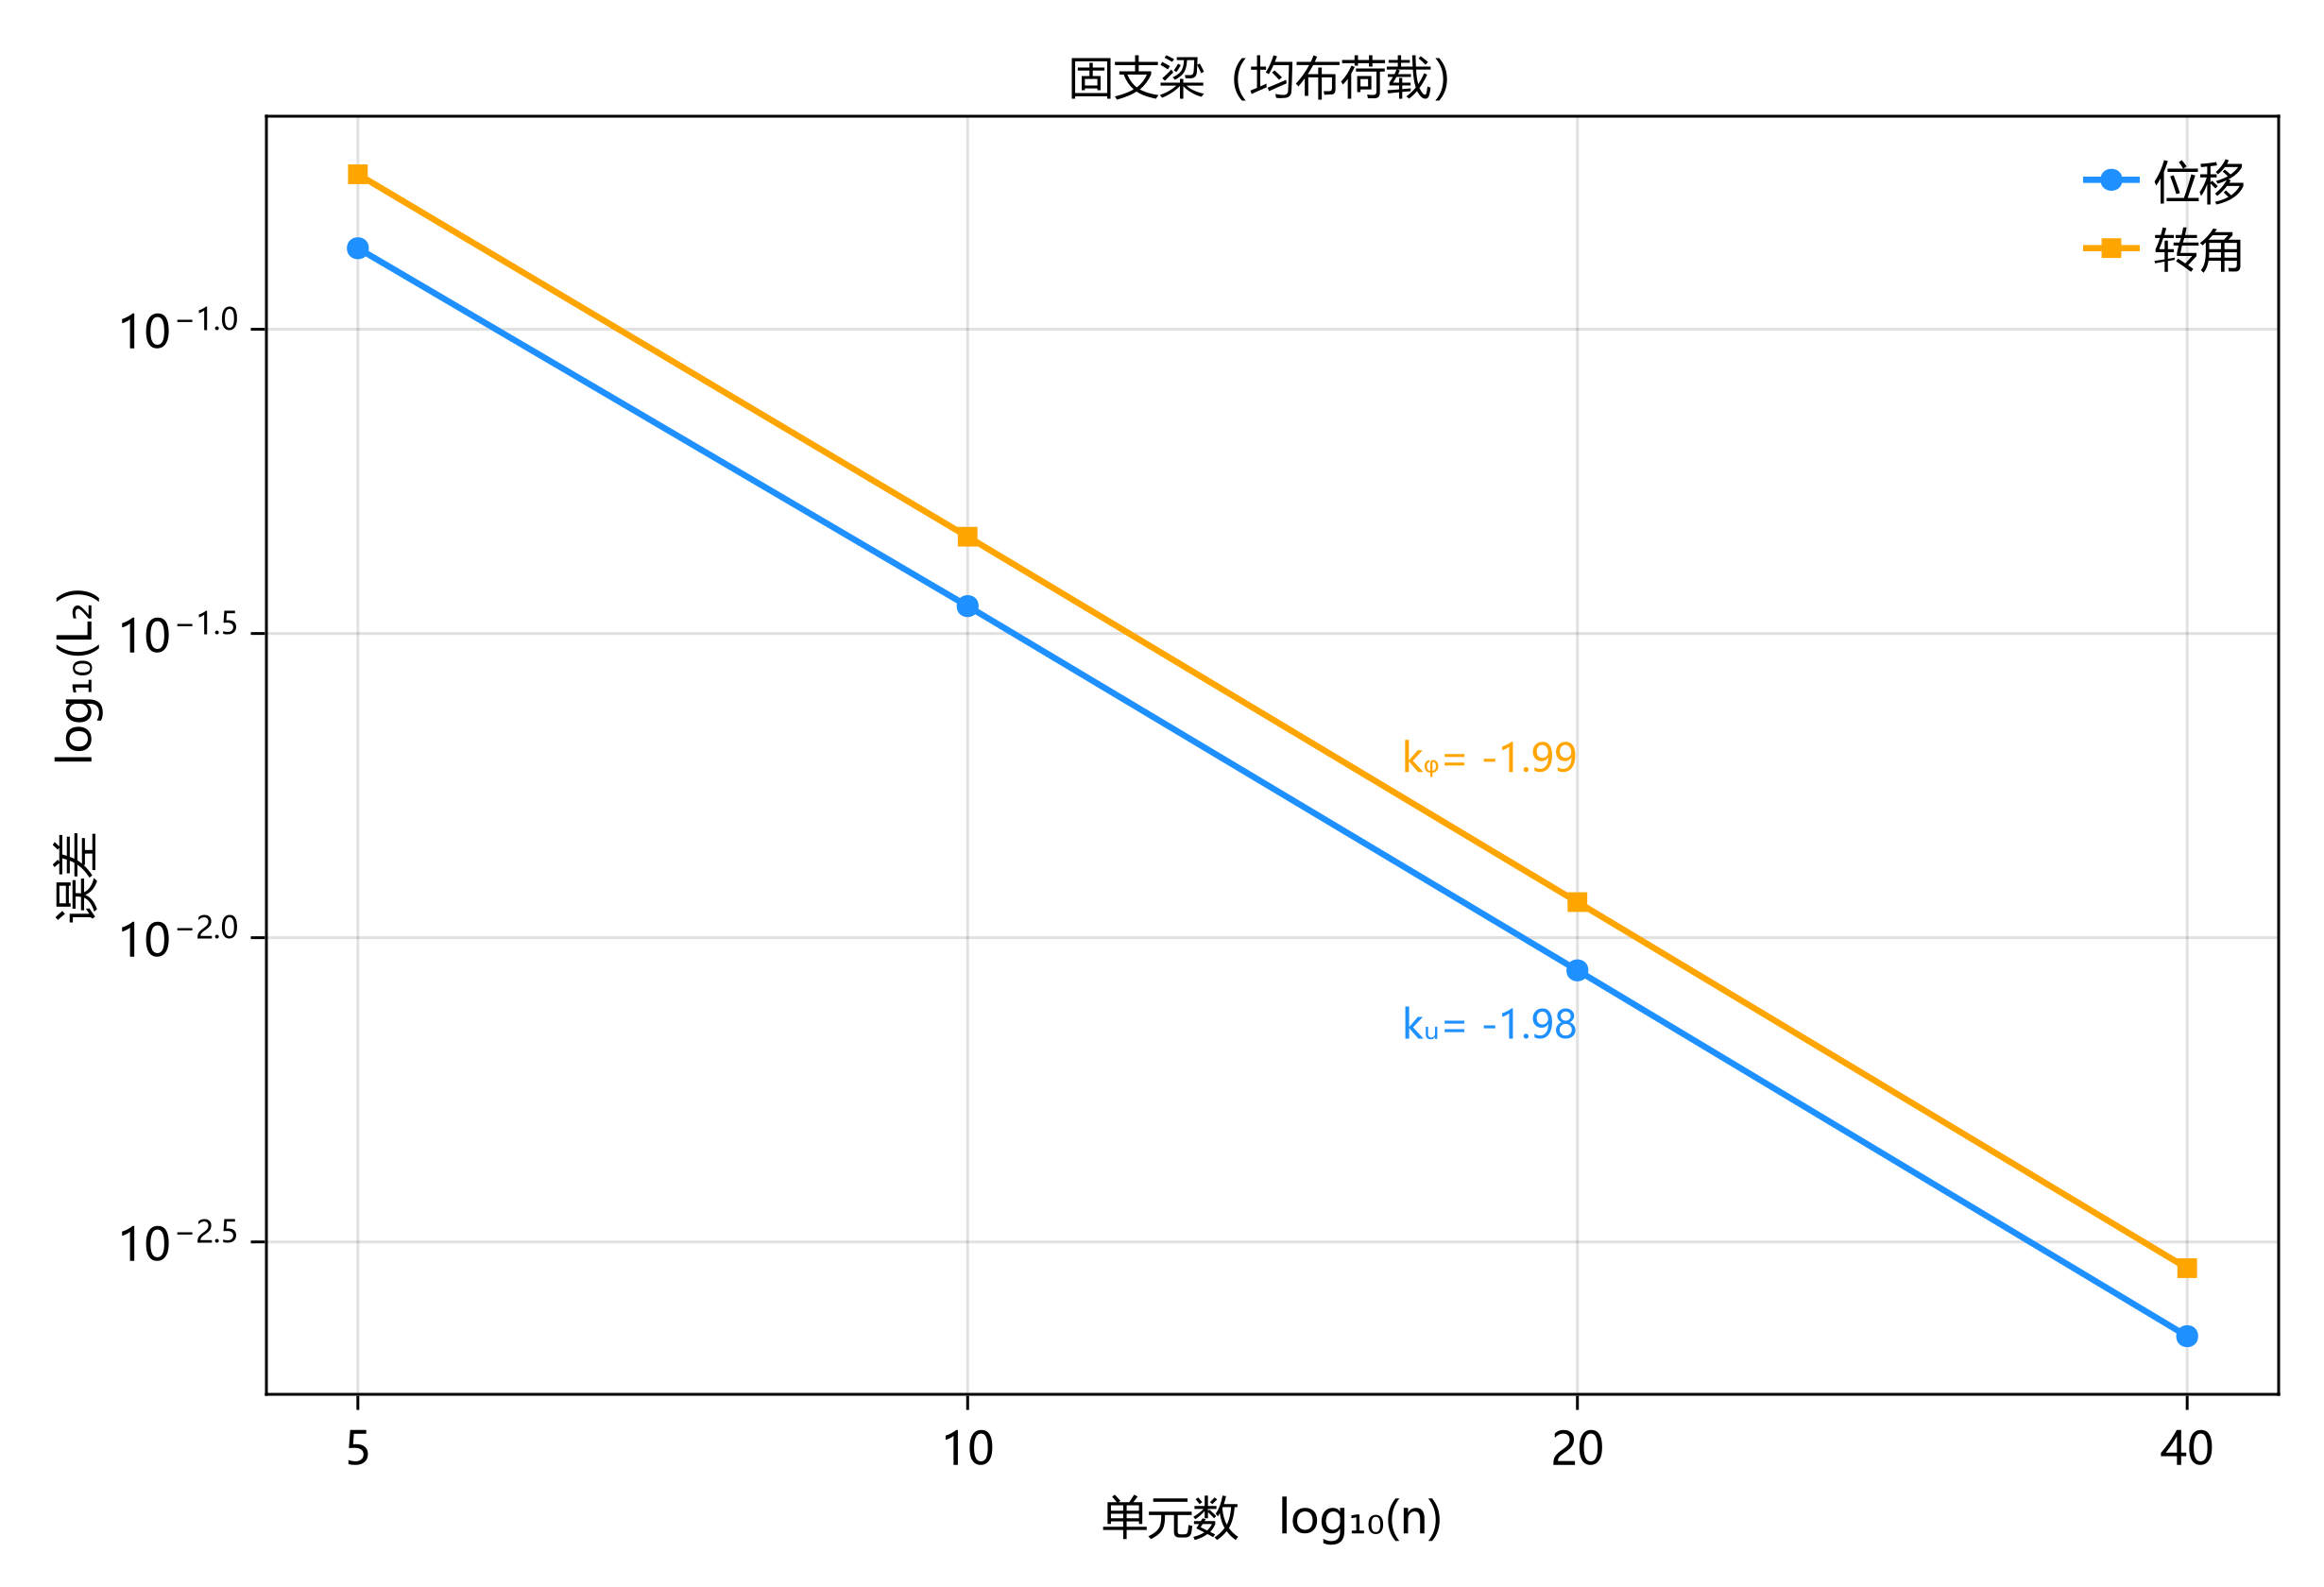
\includegraphics[width=0.78\textwidth]{fixed/l2_error.png}
\caption{固支梁均布荷载下的相对 $L_2$ 误差收敛（$n=5,10,20,40$；
位移拟合斜率 $k_u=-1.98$，转角 $k_\varphi=-1.99$）}
\label{fig:fixed-q}
\end{figure}

\begin{figure}[H]
\centering
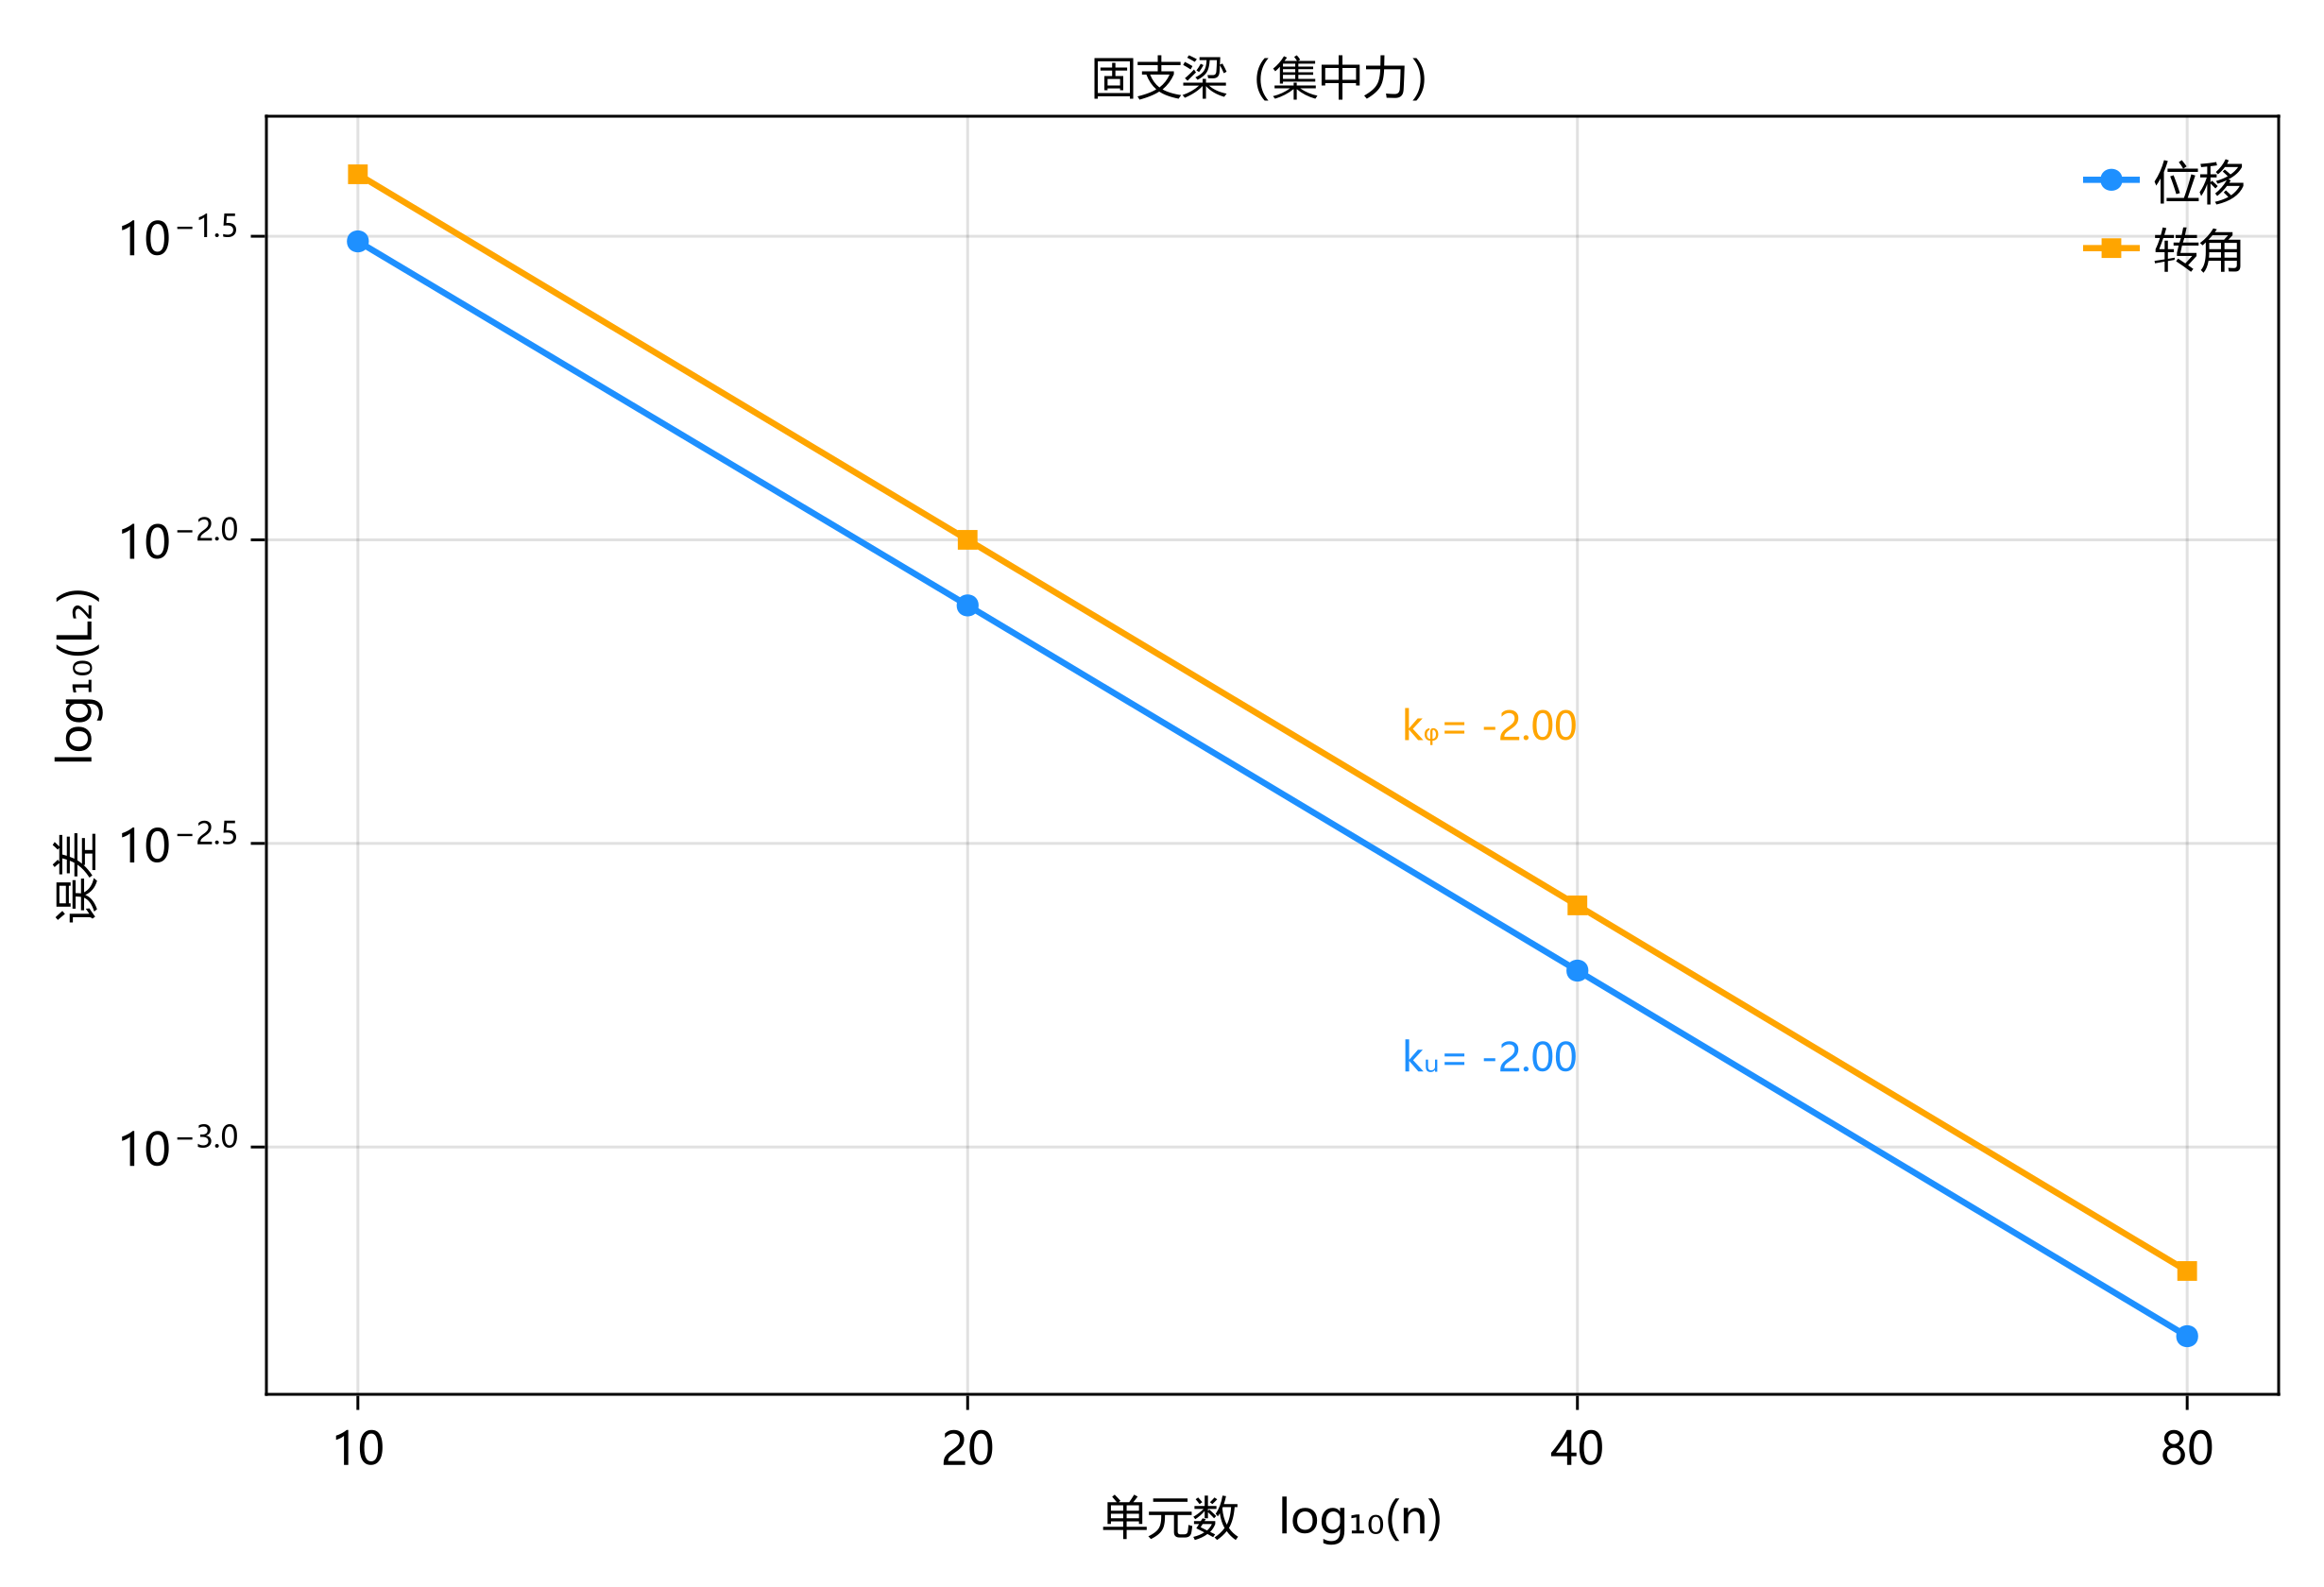
\includegraphics[width=0.78\textwidth]{fixed/l2_error_P.png}
\caption{固支梁跨中集中力下的相对 $L_2$ 误差收敛（$n=10,20,40,80$；
位移与转角的拟合斜率均为 $-2.00$）}
\label{fig:fixed-P}
\end{figure}

两条曲线在双对数坐标下都是直线，均布荷载下位移与转角的斜率分别为
$-1.98$ 与 $-1.99$，集中力下均为 $-2.00$。网格每加密一倍，误差约降为原来的
$1/4$，与 $O(h^2)$ 的理论最优阶一致。集中力工况从 $n=10$ 起算，是因为
$n=5$ 时跨中荷载附近的分段精确解还处于渐近前区，$5\to10$ 的表观收敛阶
偏高（约 $2.9$），不能代表渐近行为；从 $n=10$ 起斜率稳定在 $-2.00$。

\section{悬臂梁算例}

悬臂梁仅左端 $\Gamma^1$（$x=0$）固定，6 个自由度全部约束为零；
右端 $\Gamma^2$（$x=L$）自由。均布荷载通过 $\int N_Ib_i\ud x$ 施加，
集中力通过自由端的面力积分 $\int N_It_i\ud\Gamma$ 施加。

\subsection{精确解}

左端固定（$x=0$ 处 $w=0$、$\varphi=0$），右端自由。

均布荷载 $q$：
\begin{equation}\label{eq:cant-q}
w_q(x)=\frac{qx^2(6L^2-4Lx+x^2)}{24EI_{yy}}+\frac{qx(2L-x)}{2k_3GA},
\qquad
\varphi_q(x)=\frac{qx(3L^2-3Lx+x^2)}{6EI_{yy}}.
\end{equation}

自由端集中力 $P$：
\begin{equation}\label{eq:cant-P}
w_P(x)=\frac{Px^2(3L-x)}{6EI_{yy}}+\frac{Px}{k_3GA},
\qquad
\varphi_P(x)=\frac{Px(2L-x)}{2EI_{yy}}.
\end{equation}

\subsection{分片试验}

分片试验的线性场与固支梁算例相同（式~\eqref{eq:patchX}--\eqref{eq:patchZ}）。
需要说明的是，分片试验要求在整个边界上复现精确场，而一维梁的边界就是
两个端点，因此仍然在两端都施加精确场，这与悬臂梁实际“一端固定、一端自由”
的支承条件无关。悬臂梁的边值问题本身由下一小节的整梁 $L_2$ 误差验证。

\begin{table}[H]
\centering
\caption{悬臂梁分片试验结果}
\label{tab:patch-cant}
\small
\begin{tabular}{lccc}
\toprule
指标 & $X$ 方向 & $Y$ 方向 & $Z$ 方向\\
\midrule
主导位移分量 & $u_1$ & $u_2$ & $u_3$\\
\quad 分量相对 $L_2$（位移） & $7.000\times10^{-7}$ & $7.000\times10^{-7}$ & $7.000\times10^{-7}$\\
\quad 总体相对 $L_2$（位移） & $3.656\times10^{-7}$ & $3.656\times10^{-7}$ & $3.656\times10^{-7}$\\
主导转角分量 & $\varphi_1$ & $\varphi_2$ & $\varphi_3$\\
\quad 分量相对 $L_2$（转角） & $2.700\times10^{-8}$ & $2.700\times10^{-8}$ & $2.700\times10^{-8}$\\
\quad 总体相对 $L_2$（转角） & $2.091\times10^{-8}$ & $2.091\times10^{-8}$ & $2.091\times10^{-8}$\\
节点最大 $|\Delta d|$ & $1.680\times10^{-9}$ & $1.680\times10^{-9}$ & $1.680\times10^{-9}$\\
节点相对误差 & $4.200\times10^{-7}$ & $4.200\times10^{-7}$ & $4.200\times10^{-7}$\\
结论 & 通过 & 通过 & 通过\\
\bottomrule
\end{tabular}
\end{table}

三个方向的误差与固支梁完全一致（各指标的定义同表~\ref{tab:patch-fixed}），
总体相对 $L_2$ 位移误差为 $3.656\times10^{-7}$，转角误差为
$2.091\times10^{-8}$。这说明分片试验
只检验单元本身的插值能力，与外部支承条件无关；三种支承条件共用同一套
单元公式与刚度矩阵。

\subsection{$L_2$ 误差收敛}

\begin{figure}[H]
\centering
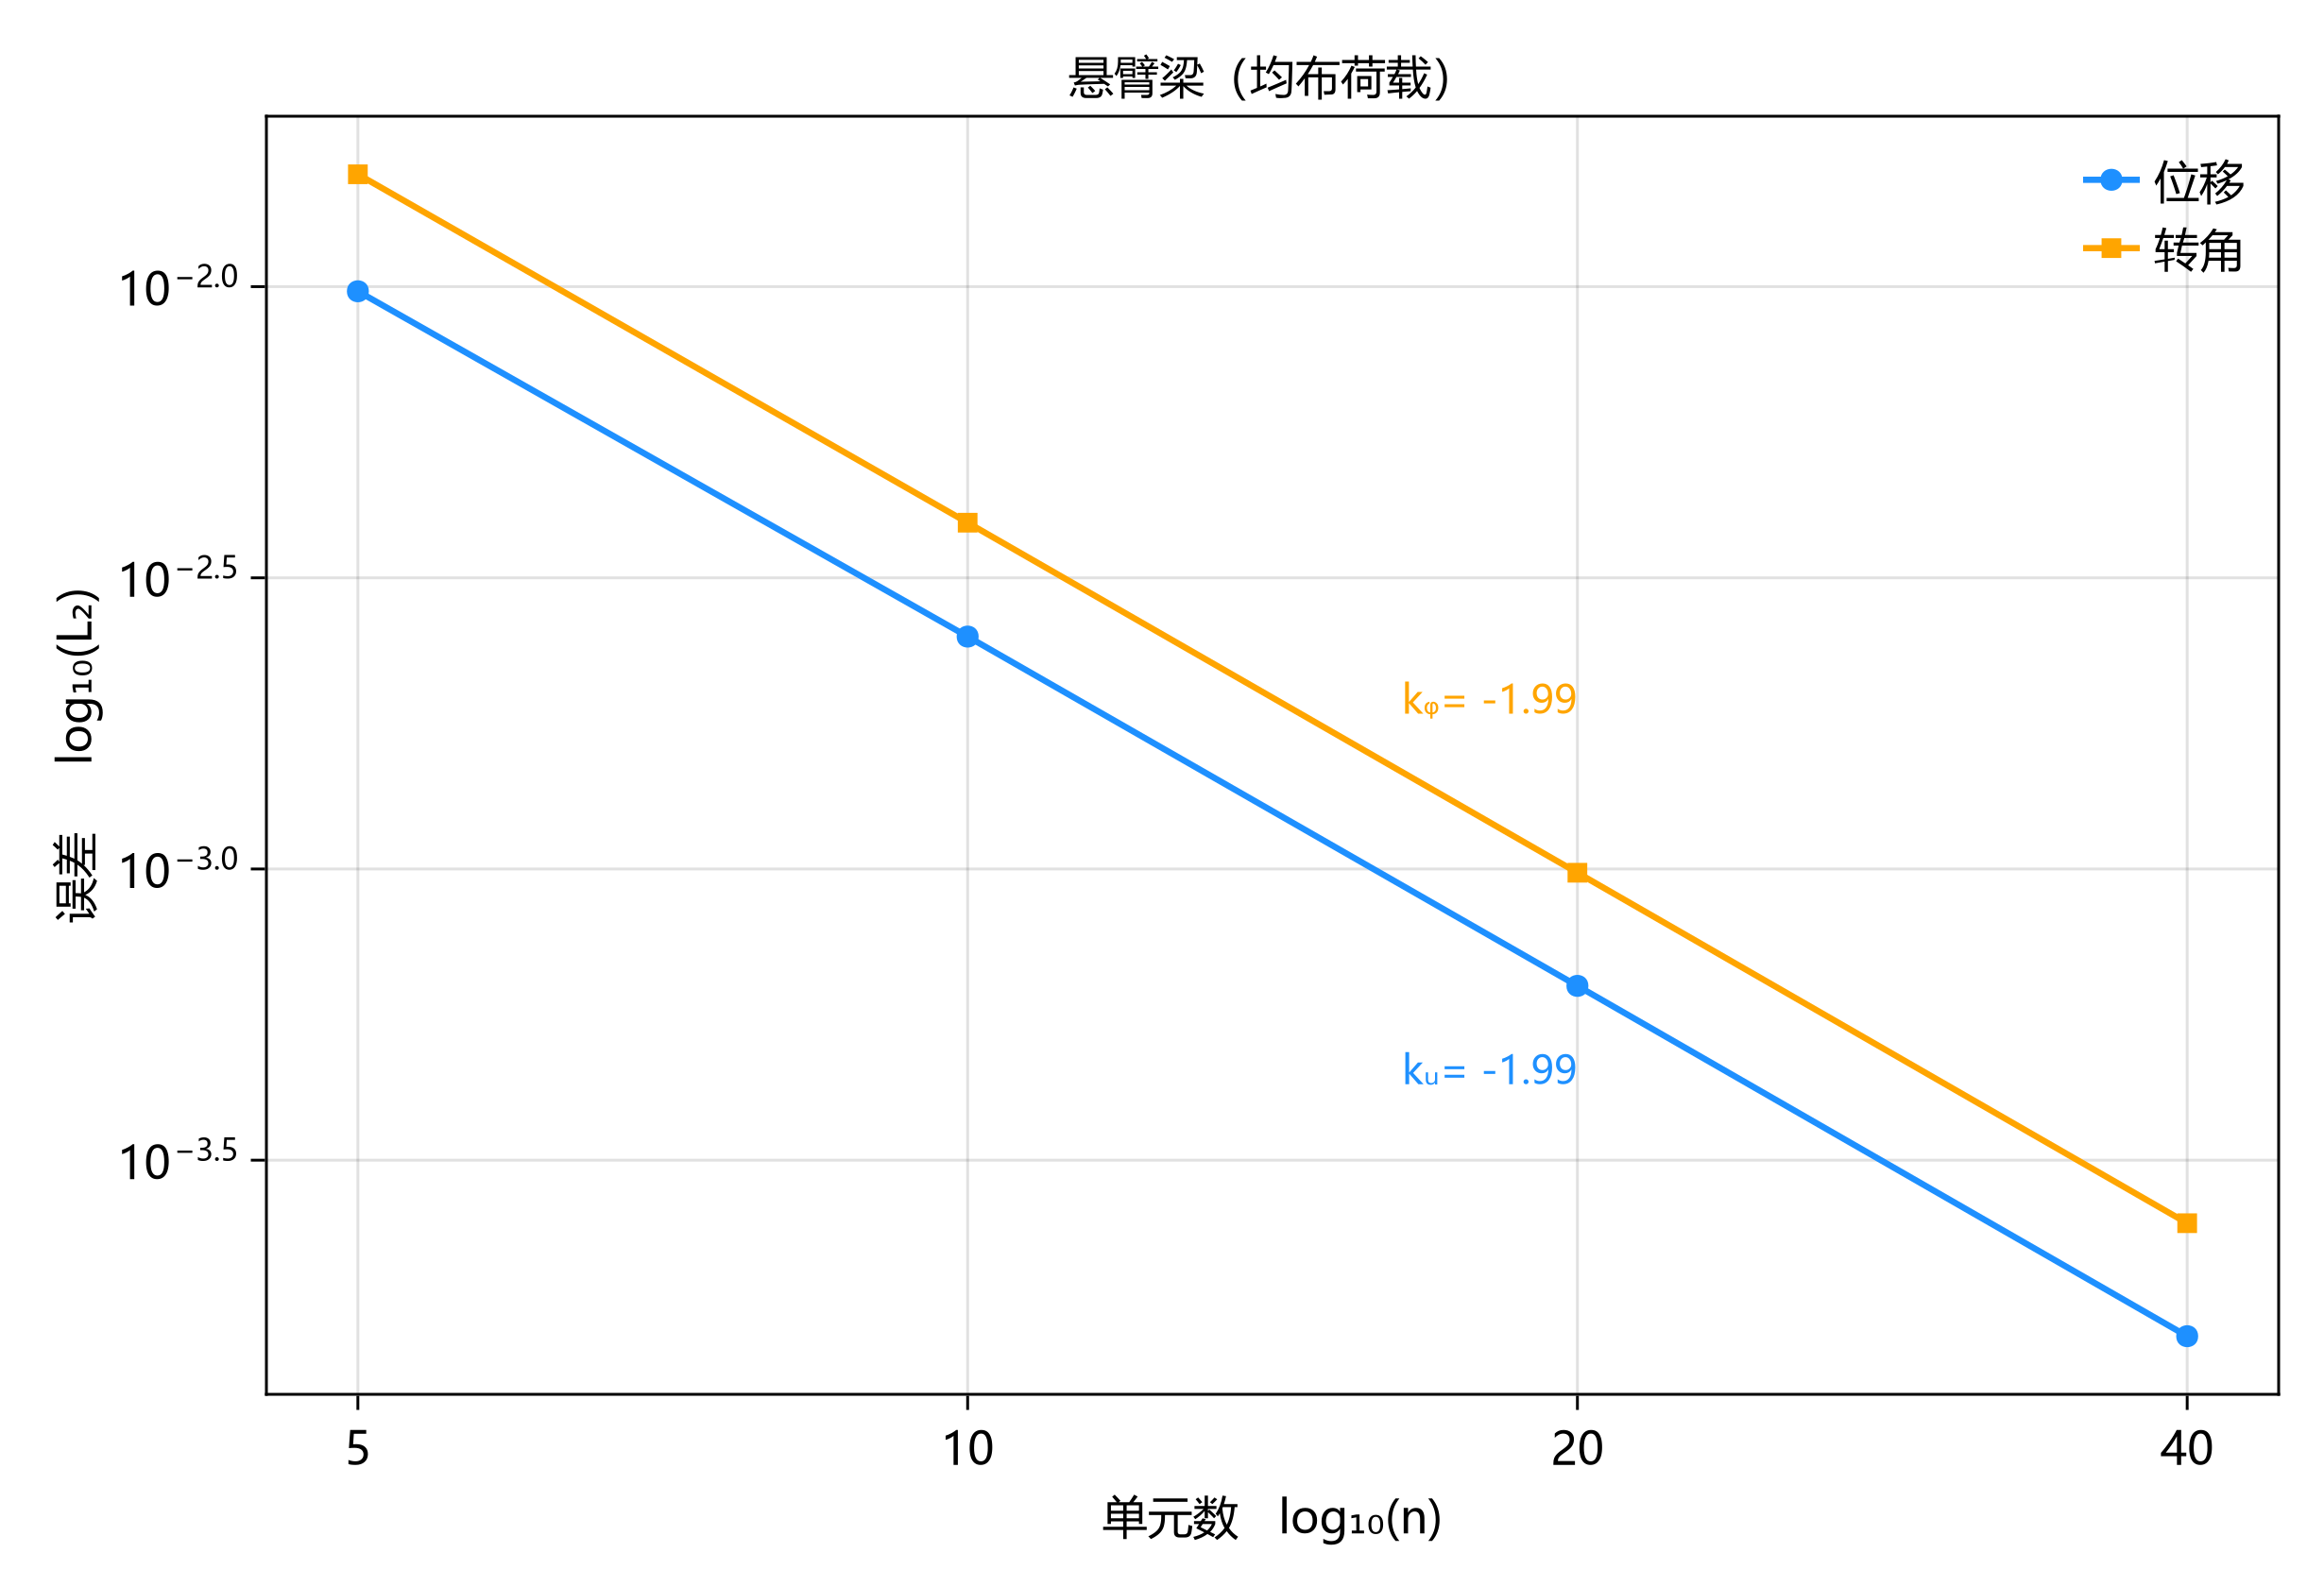
\includegraphics[width=0.78\textwidth]{cantilever/l2_error_cantilever.png}
\caption{悬臂梁均布荷载下的相对 $L_2$ 误差收敛（$n=5,10,20,40$；
位移与转角的拟合斜率均为 $-1.99$）}
\label{fig:cant-q}
\end{figure}

\begin{figure}[H]
\centering
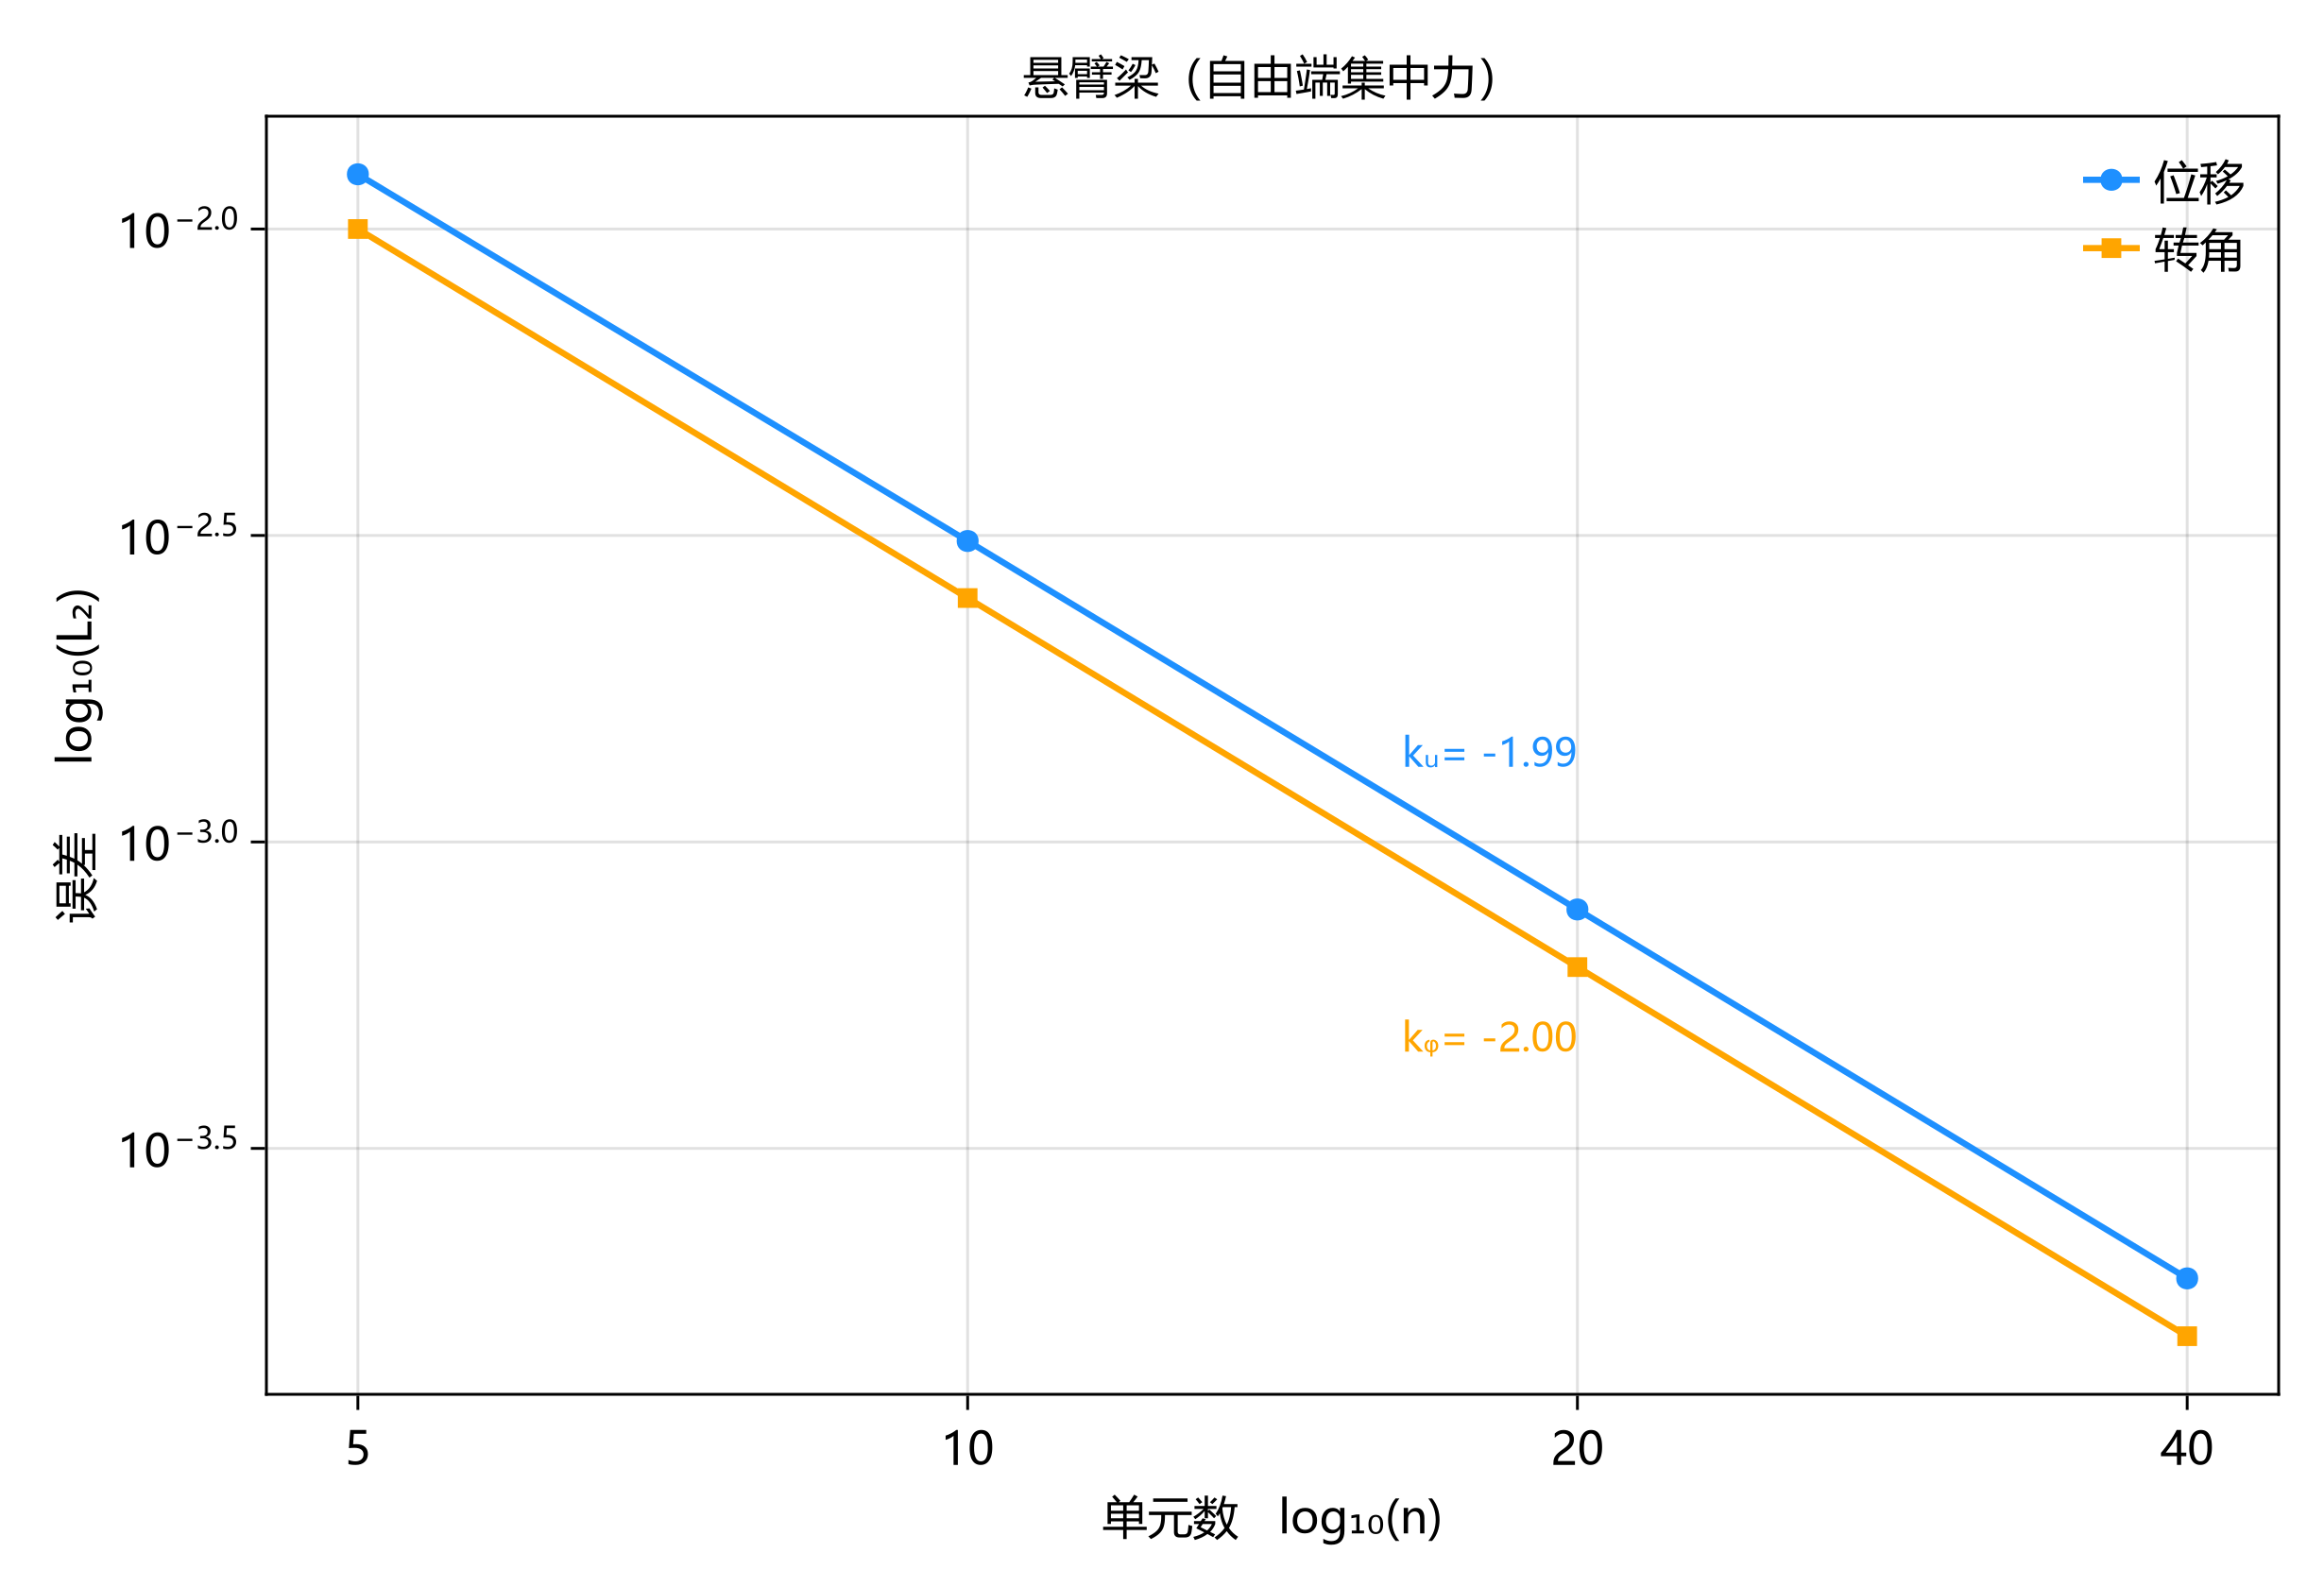
\includegraphics[width=0.78\textwidth]{cantilever/l2_error_cantilever_P.png}
\caption{悬臂梁自由端集中力下的相对 $L_2$ 误差收敛（$n=5,10,20,40$；
位移拟合斜率 $k_u=-1.99$，转角 $k_\varphi=-2.00$）}
\label{fig:cant-P}
\end{figure}

均布荷载下位移与转角的斜率均为 $-1.99$，自由端集中力下分别为 $-1.99$ 与
$-2.00$。与固支梁相比，悬臂梁只有一端提供约束，整体刚度较小、挠度较大，
但误差的收敛阶仍稳定在 $O(h^2)$，没有因自由端自然边界条件而退化。

\section{简支梁算例}

简支梁采用铰支座与滚动支座：$\Gamma^1$（$x=0$）约束
$u_1=u_2=u_3=0$ 与 $\varphi_1=0$；$\Gamma^2$（$x=L$）约束 $u_2=u_3=0$，
其余自由度自由。两端都不约束 $\varphi_3$，因此端部弯矩自然为零，这正是
“简支”的本质。约束 $\varphi_1$ 是为了消除绕梁轴的刚体扭转；两端约束 $u_3$
是为了消除侧向刚体平移与转动。由于荷载只有整体 $Y$ 向分量，$u_3$ 与
$\varphi_2$ 的响应恒为零。

\subsection{精确解}

两端简支（$x=0,L$ 处 $w=0$、弯矩为零，转角自由）。

均布荷载 $q$：
\begin{equation}\label{eq:simple-q}
w_q(x)=\frac{qx\left(L^3-2Lx^2+x^3\right)}{24EI_{yy}}+\frac{qx(L-x)}{2k_3GA},
\qquad
\varphi_q(x)=\frac{q\left(L^3-6Lx^2+4x^3\right)}{24EI_{yy}}.
\end{equation}

跨中集中力 $P$（利用对称性，$x\ge L/2$ 时用 $L-x$ 代替 $x$）：
\begin{equation}\label{eq:simple-P}
w_P(x)=
\begin{cases}
\dfrac{Px\left(3L^2-4x^2\right)}{48EI_{yy}}+\dfrac{Px}{2k_3GA}, & 0\le x\le \dfrac{L}{2},\\[8pt]
\dfrac{P(L-x)\left(3L^2-4(L-x)^2\right)}{48EI_{yy}}+\dfrac{P(L-x)}{2k_3GA}, & \dfrac{L}{2}\le x\le L,
\end{cases}
\end{equation}
\begin{equation}\label{eq:simple-P-phi}
\varphi_P(x)=
\begin{cases}
\dfrac{P\left(L^2-4x^2\right)}{16EI_{yy}}, & 0\le x\le \dfrac{L}{2},\\[8pt]
-\dfrac{P\left(L^2-4(L-x)^2\right)}{16EI_{yy}}, & \dfrac{L}{2}\le x\le L.
\end{cases}
\end{equation}

\subsection{分片试验}

分片试验的线性场与前面两个算例相同，仍在两端施加精确场。结果列于
表~\ref{tab:patch-simple}。

\begin{table}[H]
\centering
\caption{简支梁分片试验结果}
\label{tab:patch-simple}
\small
\begin{tabular}{lccc}
\toprule
指标 & $X$ 方向 & $Y$ 方向 & $Z$ 方向\\
\midrule
主导位移分量 & $u_1$ & $u_2$ & $u_3$\\
\quad 分量相对 $L_2$（位移） & $7.000\times10^{-7}$ & $7.000\times10^{-7}$ & $7.000\times10^{-7}$\\
\quad 总体相对 $L_2$（位移） & $3.656\times10^{-7}$ & $3.656\times10^{-7}$ & $3.656\times10^{-7}$\\
主导转角分量 & $\varphi_1$ & $\varphi_2$ & $\varphi_3$\\
\quad 分量相对 $L_2$（转角） & $2.700\times10^{-8}$ & $2.700\times10^{-8}$ & $2.700\times10^{-8}$\\
\quad 总体相对 $L_2$（转角） & $2.091\times10^{-8}$ & $2.091\times10^{-8}$ & $2.091\times10^{-8}$\\
节点最大 $|\Delta d|$ & $1.680\times10^{-9}$ & $1.680\times10^{-9}$ & $1.680\times10^{-9}$\\
节点相对误差 & $4.200\times10^{-7}$ & $4.200\times10^{-7}$ & $4.200\times10^{-7}$\\
结论 & 通过 & 通过 & 通过\\
\bottomrule
\end{tabular}
\end{table}

三个方向的节点相对误差均为 $4.200\times10^{-7}$，总体相对 $L_2$ 位移误差
$3.656\times10^{-7}$、转角误差 $2.091\times10^{-8}$，与固支梁、悬臂梁
完全一致（各指标的定义同表~\ref{tab:patch-fixed}）。简支支座虽然只约束
部分自由度，但分片试验在两端施加的是完整的
精确场，因此结果不受支座类型影响。

\subsection{$L_2$ 误差收敛}

\begin{figure}[H]
\centering
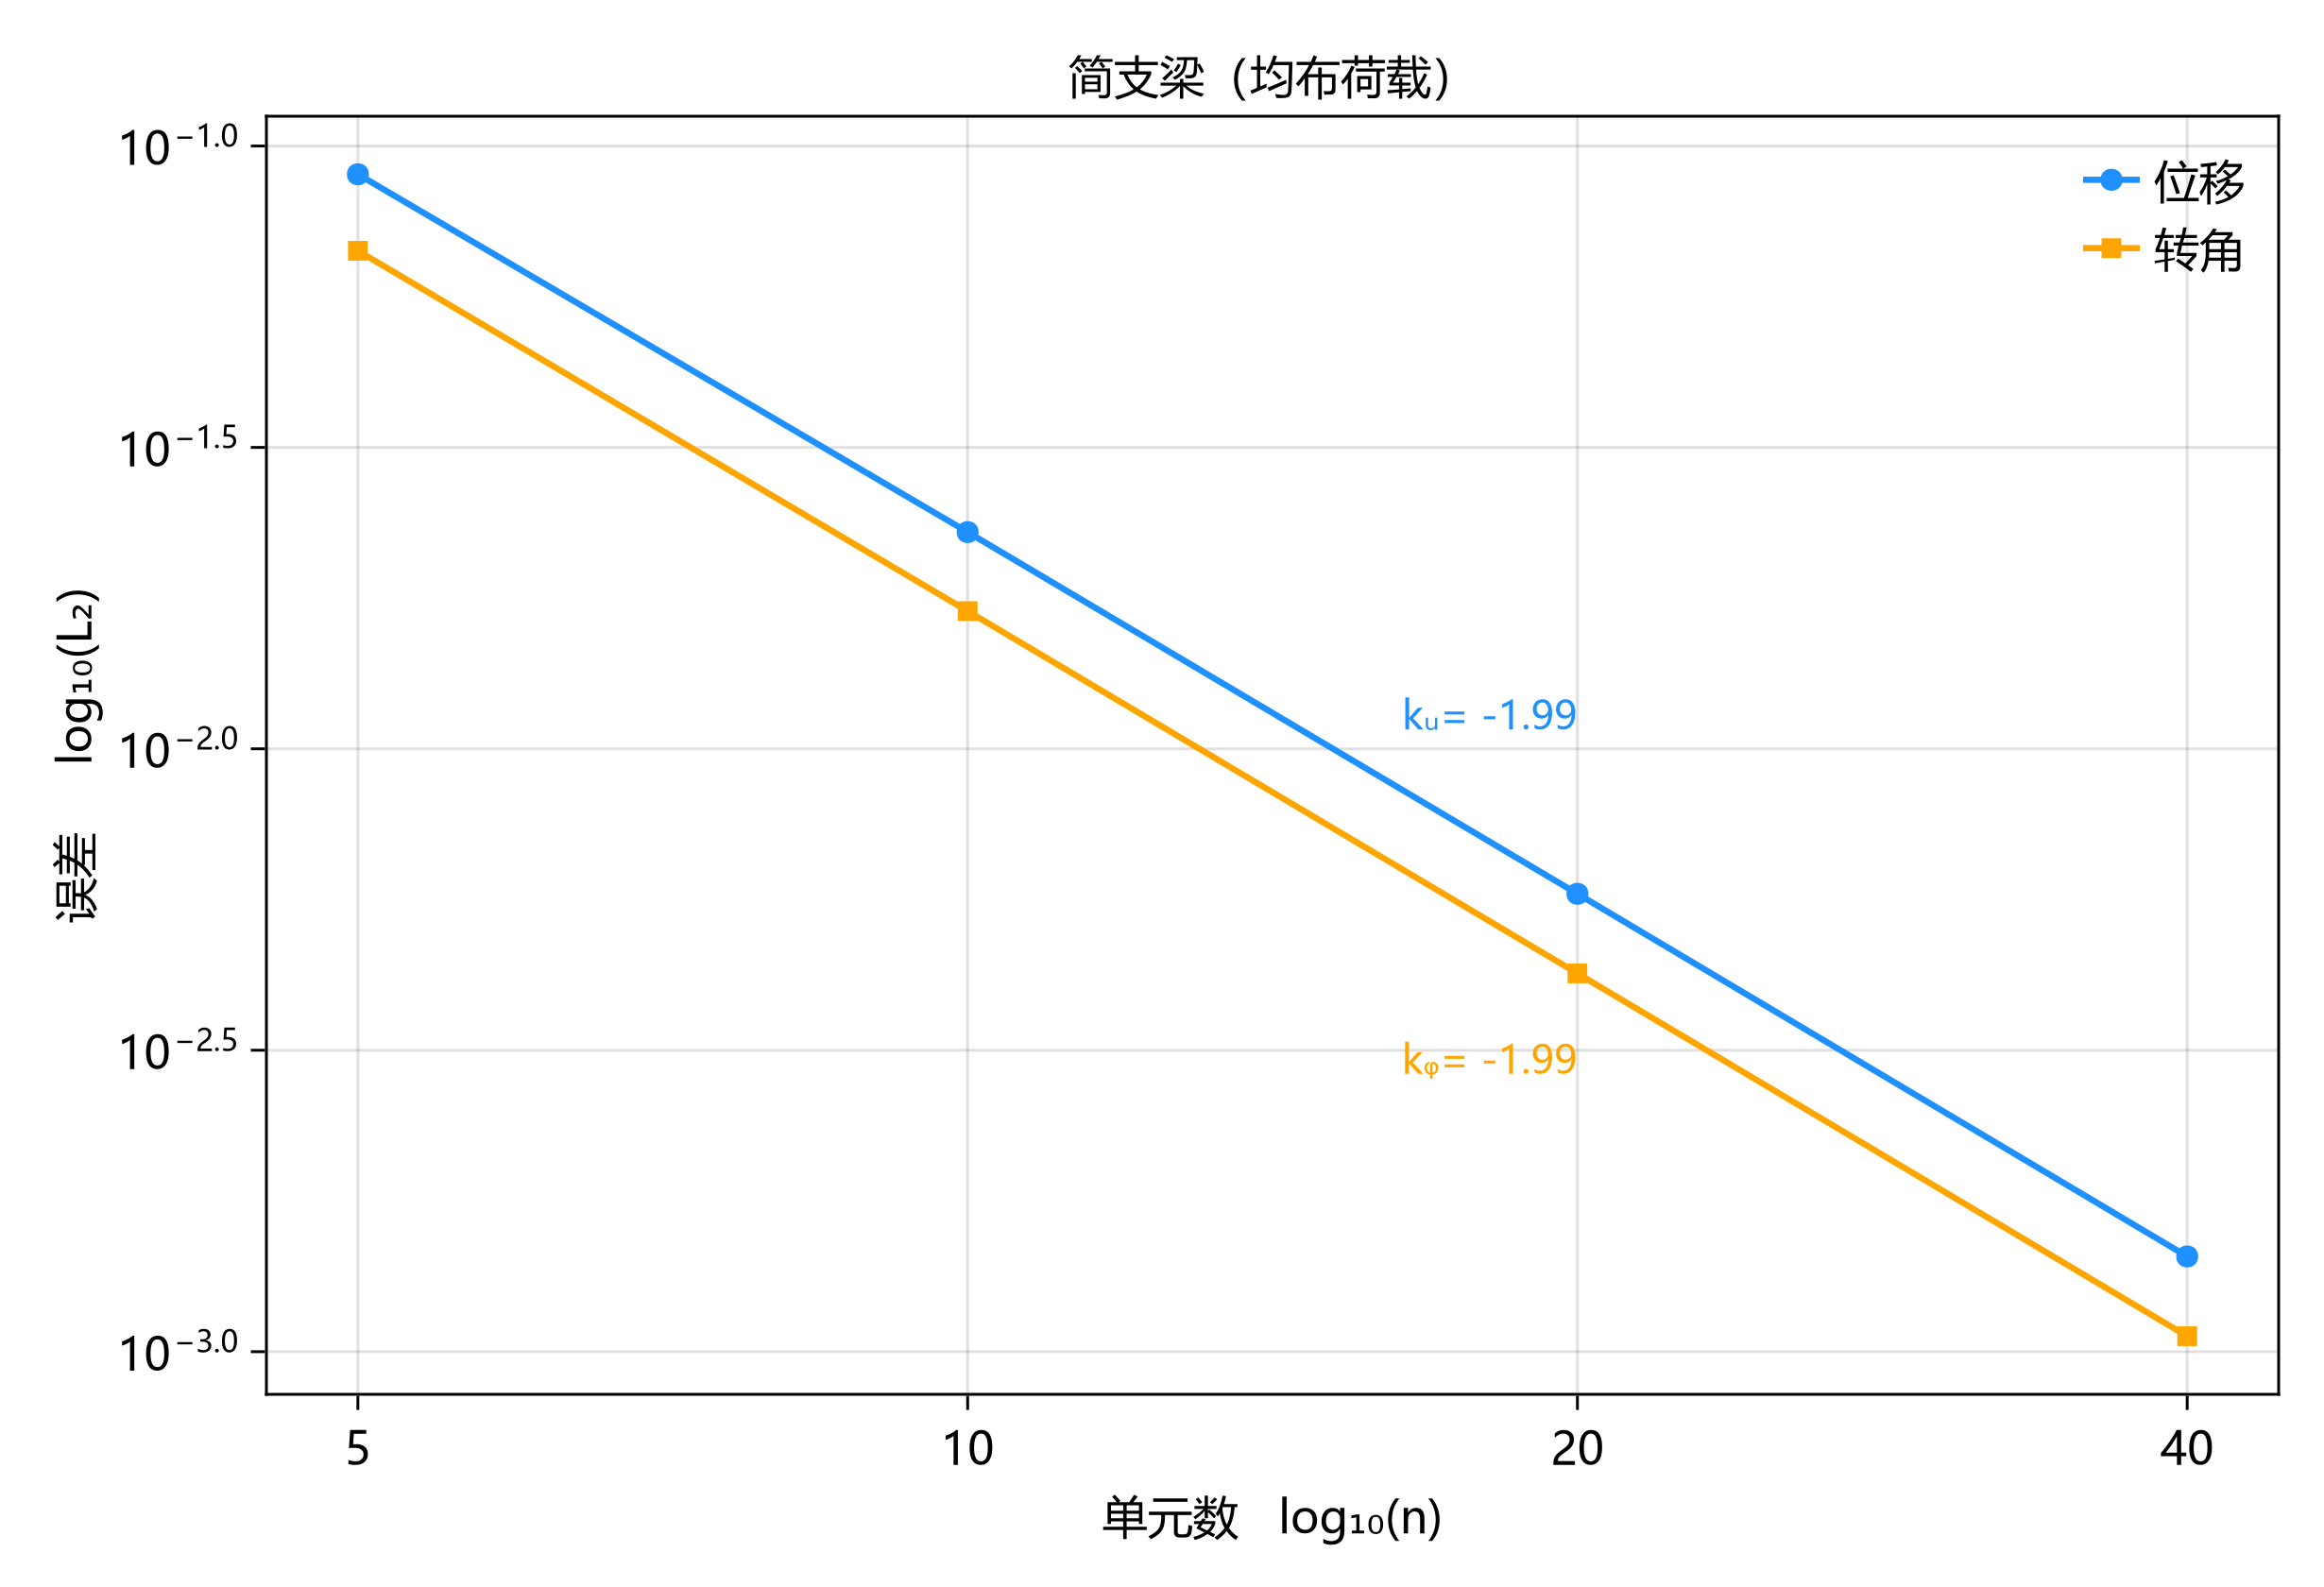
\includegraphics[width=0.78\textwidth]{simple/l2_error_simple.png}
\caption{简支梁均布荷载下的相对 $L_2$ 误差收敛（$n=5,10,20,40$；
位移与转角的拟合斜率均为 $-1.99$）}
\label{fig:simple-q}
\end{figure}

\begin{figure}[H]
\centering
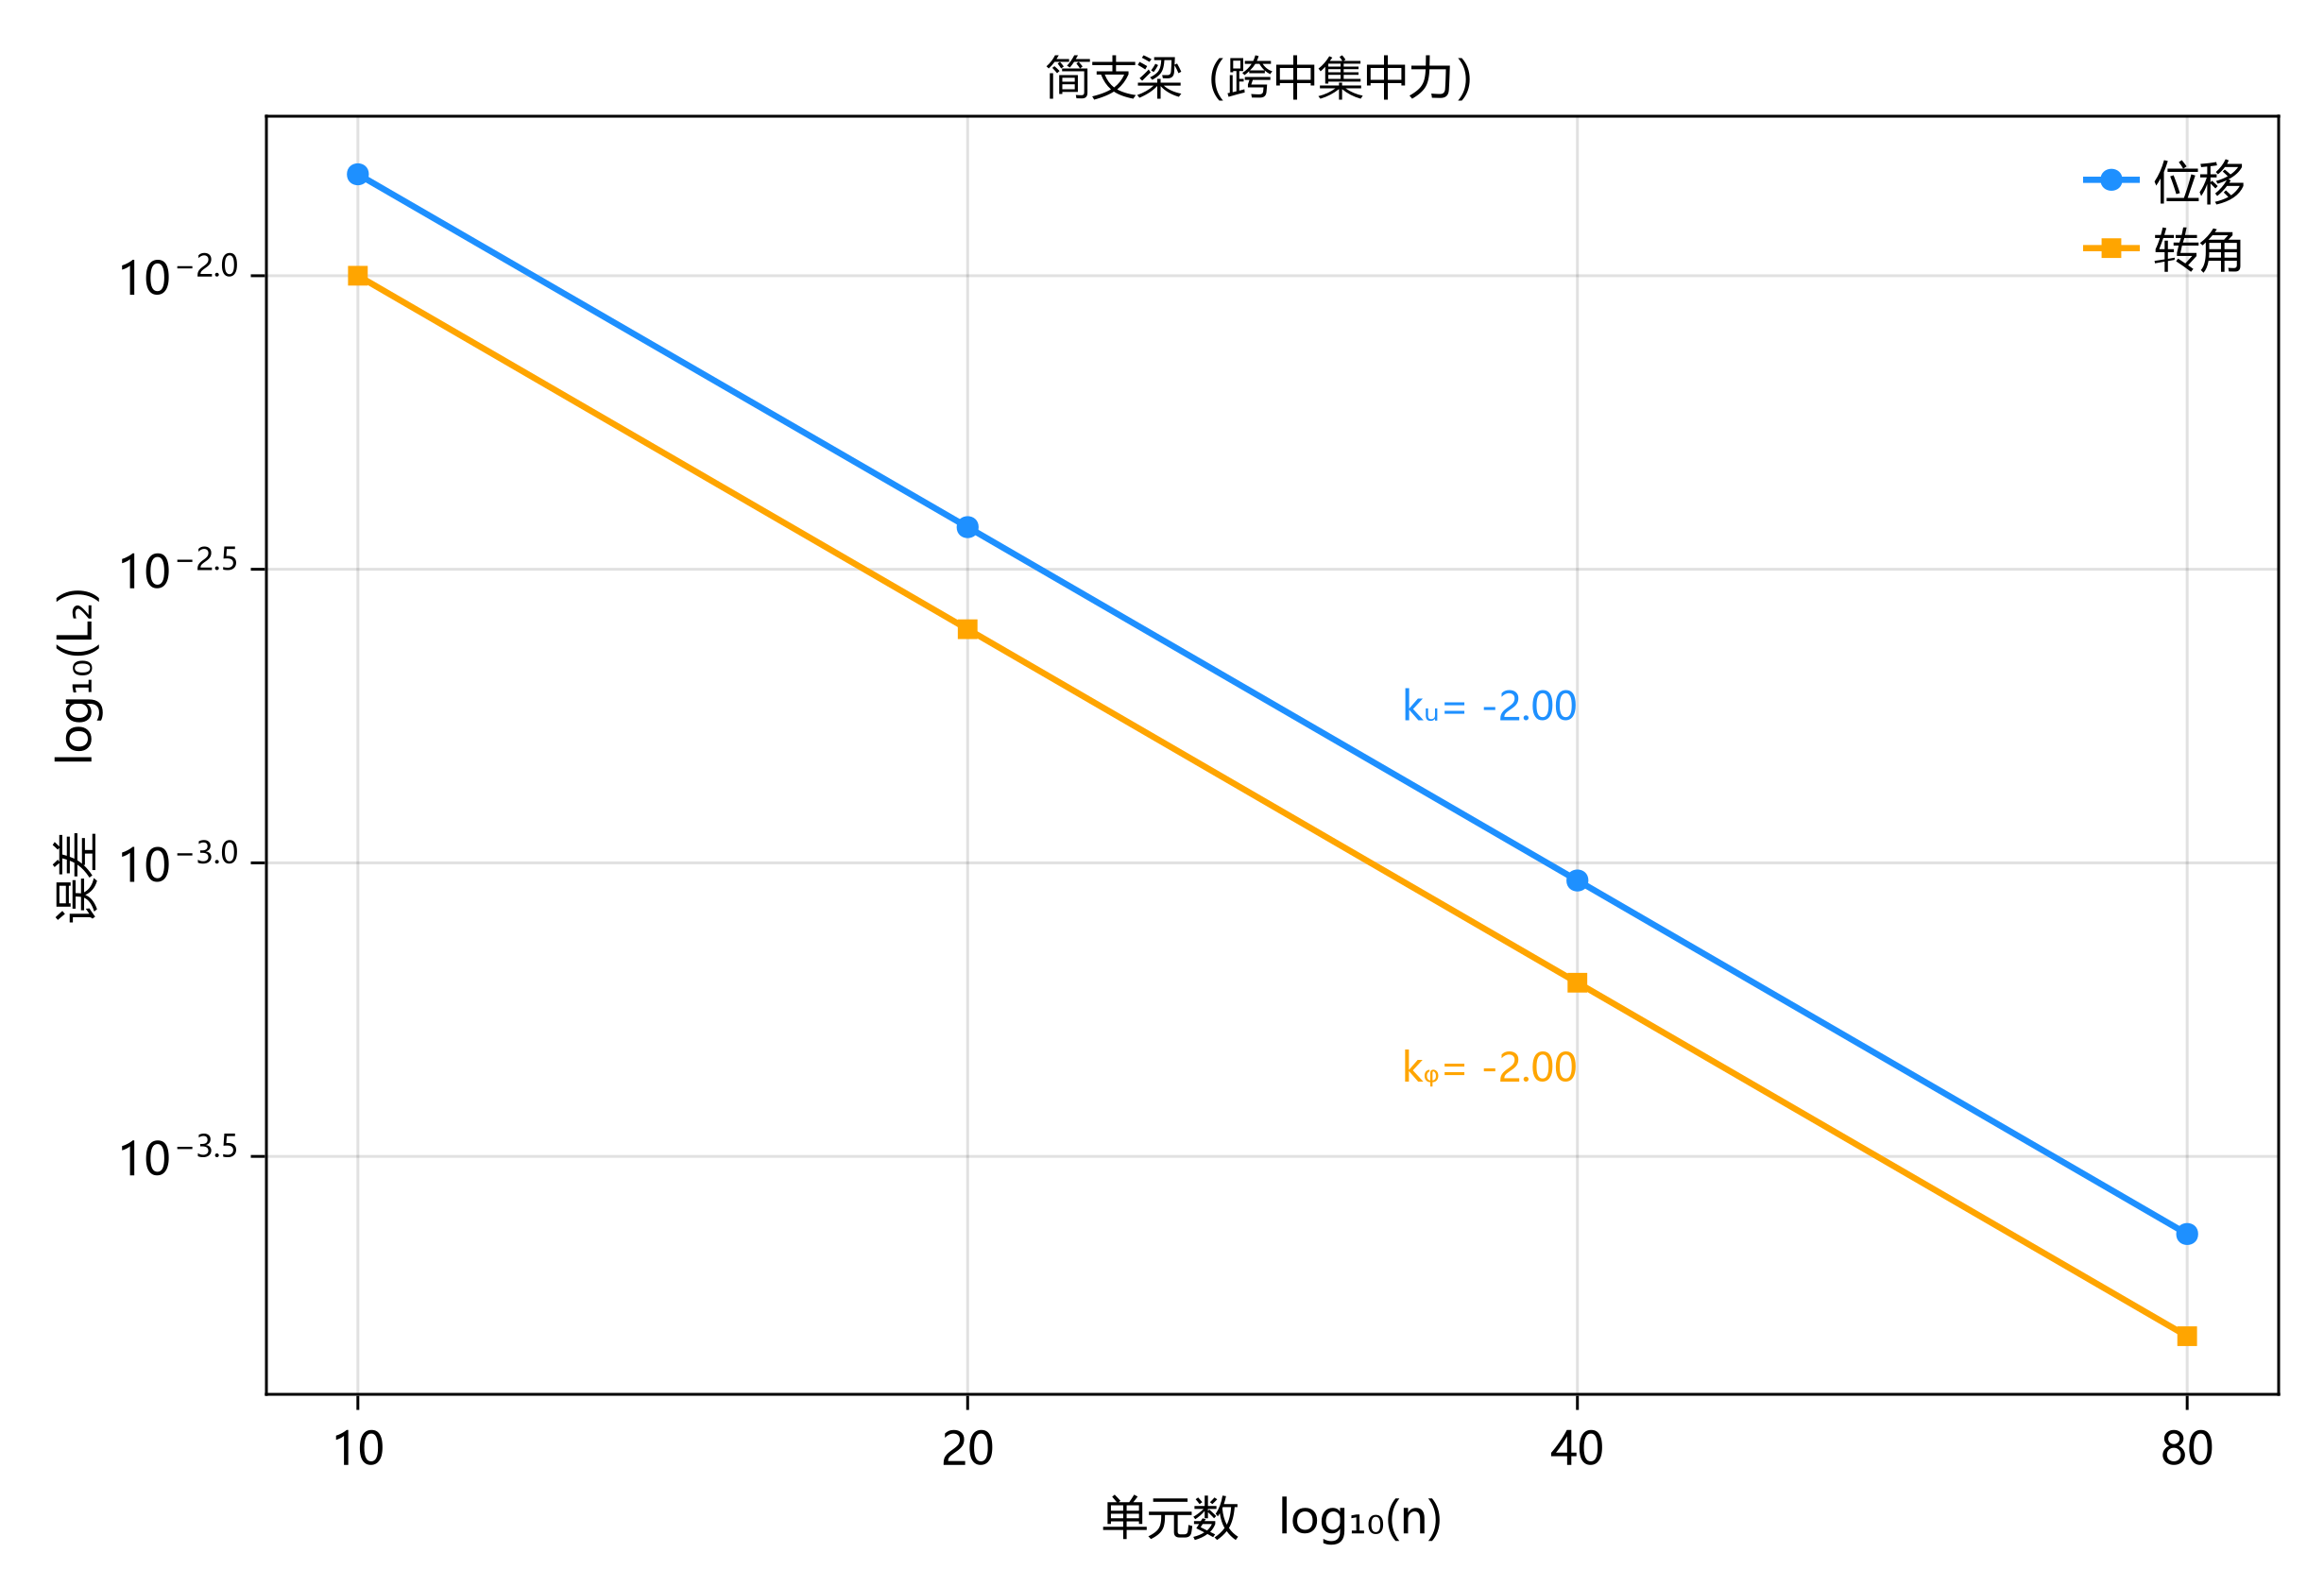
\includegraphics[width=0.78\textwidth]{simple/l2_error_simple_P.png}
\caption{简支梁跨中集中力下的相对 $L_2$ 误差收敛（$n=10,20,40,80$；
位移与转角的拟合斜率均为 $-2.00$）}
\label{fig:simple-P}
\end{figure}

均布荷载下两条曲线的斜率均为 $-1.99$；跨中集中力下均为 $-2.00$，
且网格从 $n=10$ 到 $n=80$ 时误差从 $1.489\times10^{-2}$ 降到
$2.333\times10^{-4}$，共下降约 64 倍，等于 $8^2$，与二阶收敛完全吻合。
简支梁的误差常数比固支梁、悬臂梁更大（$n=10$ 时相对 $L_2$ 约
$10^{-2}$，而前两者约 $10^{-3}$），原因是简支端弯矩为零属于自然边界条件，
只在弱形式意义下满足，端部转角误差的常数较大；但这只影响直线的截距，
不影响斜率，收敛阶仍为 $O(h^2)$。

\section{结果汇总与结论}

表~\ref{tab:summary} 汇总了三个算例在两种荷载下的拟合斜率。

\begin{table}[H]
\centering
\caption{各算例 $L_2$ 误差的双对数拟合斜率}
\label{tab:summary}
\begin{tabular}{llcc}
\toprule
算例 & 荷载 & 位移斜率 $k_u$ & 转角斜率 $k_\varphi$\\
\midrule
固支梁 & 均布 $q$ & $-1.98$ & $-1.99$\\
固支梁 & 跨中集中力 $P$ & $-2.00$ & $-2.00$\\
悬臂梁 & 均布 $q$ & $-1.99$ & $-1.99$\\
悬臂梁 & 自由端集中力 $P$ & $-1.99$ & $-2.00$\\
简支梁 & 均布 $q$ & $-1.99$ & $-1.99$\\
简支梁 & 跨中集中力 $P$ & $-2.00$ & $-2.00$\\
\bottomrule
\end{tabular}
\end{table}

由理论推导与数值结果可以得到以下结论：
\begin{enumerate}[leftmargin=2em,itemsep=3pt]
  \item 基于三维 Timoshenko 梁理论推导的两节点 Seg2 单元，每个节点 6 个自由度，
        其弱形式、刚度子块与坐标变换公式均已在第 1--6 节给出。采用形心主轴
        坐标系时，轴向、扭转与两个弯曲模式相互解耦。
  \item 单元通过了一点减缩积分消除剪切自锁。分片试验表明，$X$、$Y$、$Z$
        三个方向的线性场都能被精确复现，节点相对误差约 $4.2\times10^{-7}$，
        全域相对 $L_2$ 位移误差约 $3.7\times10^{-7}$，验证了单元的完备性与
        一致性。
  \item 固支梁、悬臂梁与简支梁在均布荷载和集中荷载下的位移、转角
        $L_2$ 误差都在双对数坐标中呈直线，斜率稳定在 $-2$ 附近，
        对应收敛阶 $p\approx2$，即 $O(h^2)$ 的最优收敛率。
  \item 三种支承条件的误差常数不同：简支梁最大，悬臂梁次之，固支梁最小。
        这与边界约束的强弱以及自然边界条件的实现方式一致，但不影响收敛阶。
  \item 由于分片试验的三个方向结果完全一致，且 $X$、$Y$、$Z$ 梁的坐标变换
        都通过验证，说明局部坐标到整体坐标的转换（包括 $Z$ 梁的特殊分支）
        实现正确。
\end{enumerate}

本报告的 $L_2$ 误差针对位移与转角。弯矩、剪力等内力通常比位移
低一阶收敛（$L_2$ 范数下多为 $O(h)$）。

\end{document}
